\documentclass{article}

\usepackage[spanish,es-tabla]{babel}
\usepackage[utf8]{inputenc}
\usepackage[T1]{fontenc}
\usepackage{listings}
\usepackage{graphicx}
\usepackage[table,xcdraw]{xcolor}
\usepackage{multirow}
\usepackage[table,xcdraw]{xcolor}
\usepackage{array}



\begin{document}
	
	%%% Portada %%%
	\begin{titlepage}
		\centering
		{\huge\textbf{SIMULACIÓN DE SISTEMAS \\ Práctica 2:\\ \vspace{0.5cm} Modelos de Monte Carlo. Generadores de datos}} \\
		
		\vspace{2cm}
		\begin{figure}[htb]
			\centering
			\includegraphics[width=400pt]{../logo_ugr.png}
		\end{figure}
		\vspace{3cm}
		{\huge Sergio Aguilera Ramírez} \\
		\vspace{1cm}
		{\large 26 de octubre de 2019}
		
	\end{titlepage}
	
	
	%%% Índice %%%
	
	\huge\textbf{Índice}
	\Large\begin{enumerate}
		\item\textbf{Capitulo 1: Mi Segundo Modelo de Simulación de
			Monte Carlo}
		\begin{enumerate}\large
			\item Modelización por Monte Carlo
				\begin{enumerate}
					\item Distribución A
					\item Distribución B
					\item Distribución C
				\end{enumerate}
			
			\item Modificaciones del modelo
		\end{enumerate}
		
		\item\textbf{Capitulo 2: Generadores de Datos}
		\begin{enumerate}\large
			\item Mejorando los Generadores
			\item Generadores conguracionales
		\end{enumerate}
	\end{enumerate}

	\newpage
	
	\Large\underline{\textbf{Capitulo 1: Mi Segundo Modelo de Simulación de Monte Carlo}} \\
	
	\textbf{1.1) - Modelización por Monte Carlo} \\
	
	\normalsize En esta sección vamos a realizar pruebas sobre las diferentes distribuciones aportadas en el guión de prácticas. En las tres secciones se ha utilizado el rango [0,100] para la asignación del valor de s. Además, los valores utilizados para "veces" son 100, 1000, 5000 y 100000. En las secciones se mostrarán gráficas que representarán las salidas obtenidos por el programa mediante los diferentes valores de los parámetros utilizados.  \\
	
	 \section*{a) - Distribución A (U(0,99))}
	 En este experimente vamos a distribuir de forma uniforme la probabilidad de demanda. Las siguientes gráficas muestran la evolución de la ganancia a lo largo de la ejecución donde el valor de 's' se va modificando. 
	 	
	 
	 \begin{figure}[h]
	 	\centering
	 	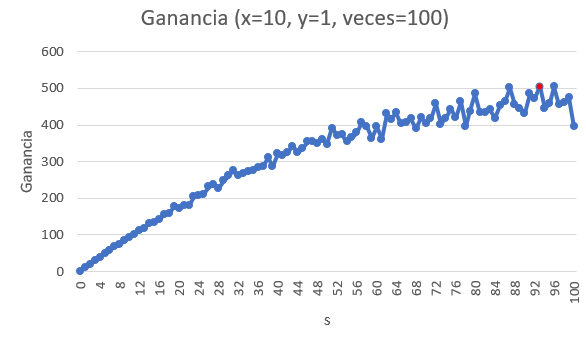
\includegraphics[width=150pt]{./graficas/10-1-100a.png}
	 	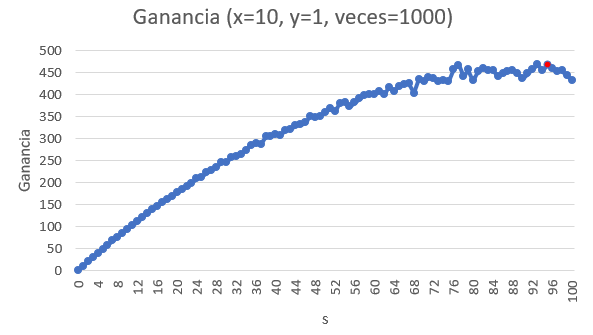
\includegraphics[width=150pt]{./graficas/10-1-1000a.png}
	 	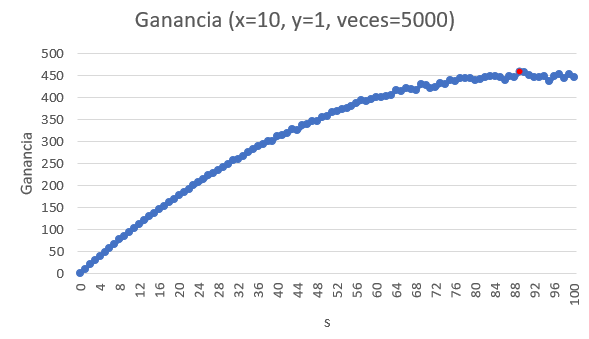
\includegraphics[width=150pt]{./graficas/10-1-5000a.png}
	 	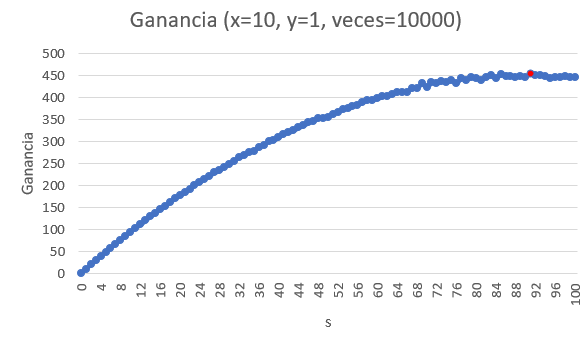
\includegraphics[width=150pt]{./graficas/10-1-10000a.png}
	 	\caption{Evolución de la Ganancia (x=10, y=5) Distribución A}
	 \end{figure} 
 
 	La Figura 1 muestra la evolución de la ganancia para un valor de x=10 y un valor de y=1, es decir, el valor de ganancia de cada producto es de 10 y la perdida por producto no vendido es de 1. vemos como las gráficas son crecientes hasta llegar a un cierto valor de 's' donde las gráficas se van estabilizando.
 	
 	\newpage
 	
 	La siguiente gráfica (Figura 2), como se ha dicho en el apartado anterior muestra la evolución de la ganancia pero con un valor de x=10 y de y=5, lo cual supone una mayor perdida sobre los productos no vendidos. Como vemos cuando 's' crece mucho la ganancia empieza a caer, esto se debe a que los productos a partir de una cierta cantidad se dejan de vender lo cual supone un gran impacto sobre la ganancia.
 
 
 	\begin{figure}[h]
 		\centering
 		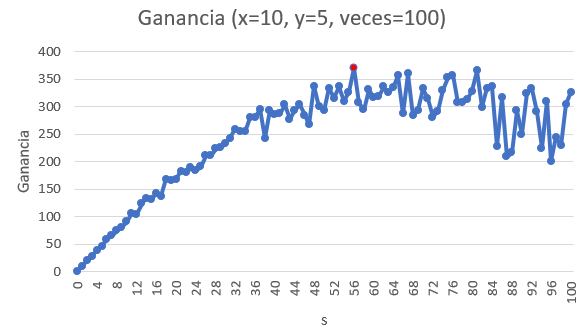
\includegraphics[width=150pt]{./graficas/10-5-100a.png}
 		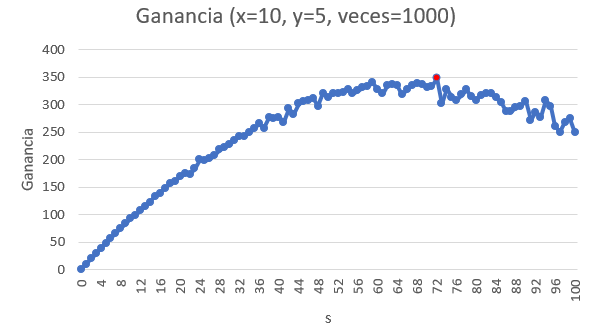
\includegraphics[width=150pt]{./graficas/10-5-1000a.png}
 		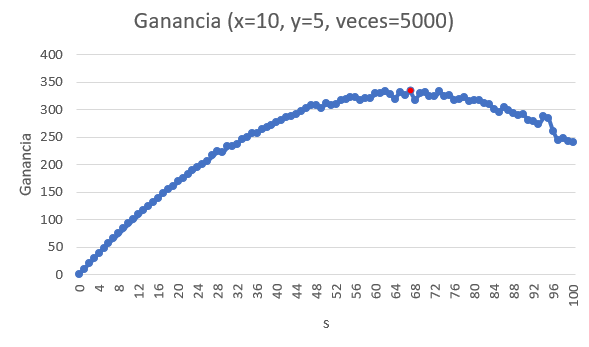
\includegraphics[width=150pt]{./graficas/10-5-5000a.png}
 		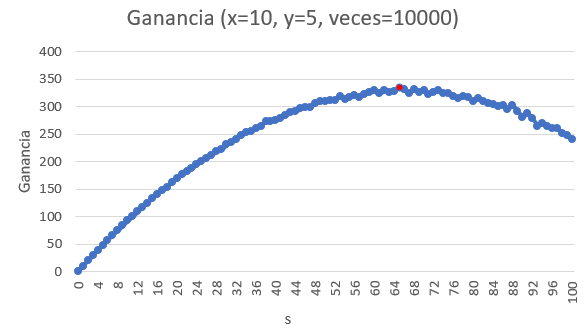
\includegraphics[width=150pt]{./graficas/10-5-10000a.png}
 		\caption{Evolución de la Ganancia (x=10, y=5) Distribución A}
 	\end{figure} 
 
  	De igual forma ocurre en la Figura 3, donde el coste de perdida es de 10. El programa con esta distribución predice que durante un periodo de tiempo más largo el valor de ganancia decaerá proporcionalmente que aumenta el valor de 's'.
	
	
	\begin{figure}[h]
		\centering
		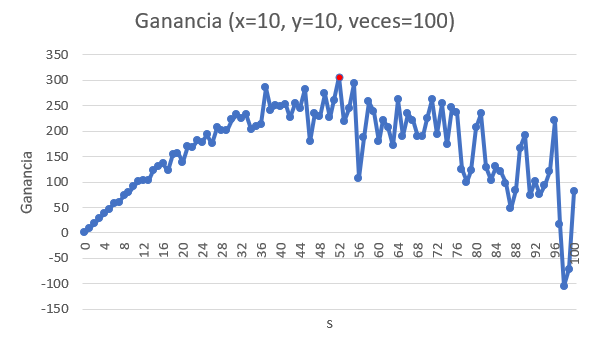
\includegraphics[width=100pt]{./graficas/10-10-100a.png}
		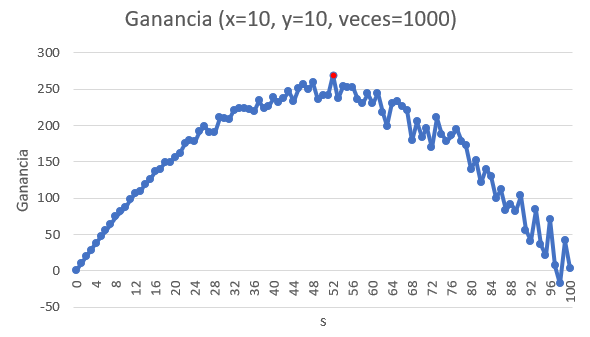
\includegraphics[width=100pt]{./graficas/10-10-1000a.png}
		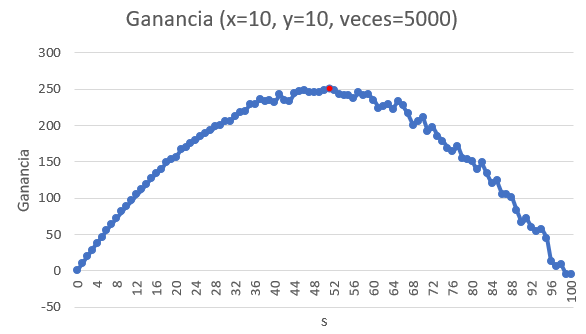
\includegraphics[width=100pt]{./graficas/10-10-5000a.png}
		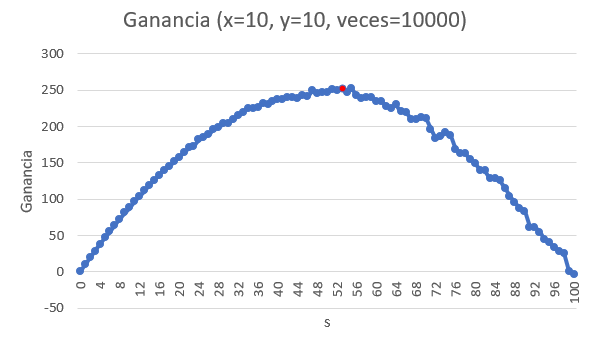
\includegraphics[width=100pt]{./graficas/10-10-10000a.png}
		\caption{Evolución de la Ganancia (x=10, y=5) Distribución A}
	\end{figure}
	
	\newpage
	
	Respecto a las gráficas anteriores se puede observar en rojo el punto cuya ganancia es la mejor obtenida en todo el proceso.
	
	
	\begin{table}[h]
		\begin{tabular}{llllll}
			\hline
			\rowcolor[HTML]{F8A102} 
			\multicolumn{1}{|l|}{\cellcolor[HTML]{F8A102}{\color[HTML]{000000} x}} & \multicolumn{1}{l|}{\cellcolor[HTML]{F8A102}{\color[HTML]{000000} y}} & \multicolumn{1}{l|}{\cellcolor[HTML]{F8A102}{\color[HTML]{000000} veces}} & \multicolumn{1}{l|}{\cellcolor[HTML]{F8A102}{\color[HTML]{000000} Mejor\_s}} & \multicolumn{1}{l|}{\cellcolor[HTML]{F8A102}{\color[HTML]{000000} Mejor\_ganancia}} & \multicolumn{1}{l|}{\cellcolor[HTML]{F8A102}{\color[HTML]{000000} Mejor\_desviacion}} \\ \hline
			\multicolumn{1}{|l|}{}                                                 & \multicolumn{1}{l|}{}                                                 & \multicolumn{1}{l|}{100}                                                  & \multicolumn{1}{l|}{93}                                                      & \multicolumn{1}{l|}{505,62}                                                         & \multicolumn{1}{l|}{292,842}                                                          \\ \cline{3-6} 
			\multicolumn{1}{|l|}{}                                                 & \multicolumn{1}{l|}{}                                                 & \multicolumn{1}{l|}{1000}                                                 & \multicolumn{1}{l|}{95}                                                      & \multicolumn{1}{l|}{469,872}                                                        & \multicolumn{1}{l|}{314,4571}                                                         \\ \cline{3-6} 
			\multicolumn{1}{|l|}{}                                                 & \multicolumn{1}{l|}{}                                                 & \multicolumn{1}{l|}{5000}                                                 & \multicolumn{1}{l|}{89}                                                      & \multicolumn{1}{l|}{459,4292}                                                       & \multicolumn{1}{l|}{308,1974}                                                         \\ \cline{3-6} 
			\multicolumn{1}{|l|}{\multirow{-4}{*}{10}}                             & \multicolumn{1}{l|}{\multirow{-4}{*}{1}}                              & \multicolumn{1}{l|}{10000}                                                & \multicolumn{1}{l|}{91}                                                      & \multicolumn{1}{l|}{454,5472}                                                       & \multicolumn{1}{l|}{310,8374}                                                         \\ \hline
			&                                                                       &                                                                           &                                                                              &                                                                                     &                                                                                       \\ \hline
			\multicolumn{1}{|l|}{}                                                 & \multicolumn{1}{l|}{}                                                 & \multicolumn{1}{l|}{100}                                                  & \multicolumn{1}{l|}{56}                                                      & \multicolumn{1}{l|}{371,15}                                                         & \multicolumn{1}{l|}{256,817}                                                          \\ \cline{3-6} 
			\multicolumn{1}{|l|}{}                                                 & \multicolumn{1}{l|}{}                                                 & \multicolumn{1}{l|}{1000}                                                 & \multicolumn{1}{l|}{72}                                                      & \multicolumn{1}{l|}{348,75}                                                         & \multicolumn{1}{l|}{350,5631}                                                         \\ \cline{3-6} 
			\multicolumn{1}{|l|}{}                                                 & \multicolumn{1}{l|}{}                                                 & \multicolumn{1}{l|}{5000}                                                 & \multicolumn{1}{l|}{67}                                                      & \multicolumn{1}{l|}{348,75}                                                         & \multicolumn{1}{l|}{350,5631}                                                         \\ \cline{3-6} 
			\multicolumn{1}{|l|}{\multirow{-4}{*}{10}}                             & \multicolumn{1}{l|}{\multirow{-4}{*}{5}}                              & \multicolumn{1}{l|}{10000}                                                & \multicolumn{1}{l|}{65}                                                      & \multicolumn{1}{l|}{348,75}                                                         & \multicolumn{1}{l|}{350,5631}                                                         \\ \hline
			&                                                                       &                                                                           &                                                                              &                                                                                     &                                                                                       \\ \hline
			\multicolumn{1}{|l|}{}                                                 & \multicolumn{1}{l|}{}                                                 & \multicolumn{1}{l|}{100}                                                  & \multicolumn{1}{l|}{52}                                                      & \multicolumn{1}{l|}{348,75}                                                         & \multicolumn{1}{l|}{350,5631}                                                         \\ \cline{3-6} 
			\multicolumn{1}{|l|}{}                                                 & \multicolumn{1}{l|}{}                                                 & \multicolumn{1}{l|}{1000}                                                 & \multicolumn{1}{l|}{52}                                                      & \multicolumn{1}{l|}{348,75}                                                         & \multicolumn{1}{l|}{350,5631}                                                         \\ \cline{3-6} 
			\multicolumn{1}{|l|}{}                                                 & \multicolumn{1}{l|}{}                                                 & \multicolumn{1}{l|}{5000}                                                 & \multicolumn{1}{l|}{51}                                                      & \multicolumn{1}{l|}{348,75}                                                         & \multicolumn{1}{l|}{350,5631}                                                         \\ \cline{3-6} 
			\multicolumn{1}{|l|}{\multirow{-4}{*}{10}}                             & \multicolumn{1}{l|}{\multirow{-4}{*}{10}}                             & \multicolumn{1}{l|}{10000}                                                & \multicolumn{1}{l|}{53}                                                      & \multicolumn{1}{l|}{348,75}                                                         & \multicolumn{1}{l|}{350,5631}                                                         \\ \hline
		\end{tabular}
	\caption{Resultados Distribución A}
	\end{table}

	Por otra parte, en la Tabla 1 podemos ver los mejores resultados obtenidos por los diferentes parámetros sobre esta distribución. Como he comentado anteriormente se puede ver como el mejor valor de 's' obtenido es menor conforme el valor de perdida aumenta. Los mejores resultados de ganancia si comparamos entre los resultados obtenidos para los diferentes valores de 'y' son obtenidos para el valor de perdida 1, además la desviación en esta también es menor.

	\section*{b) - Distribución B (Proporcional a 100-d)}	
	
		\normalsize En este apartado se ha utilizado una distribución proporcional a 100-d. \\
		
		\begin{figure}[htb]
			\centering
			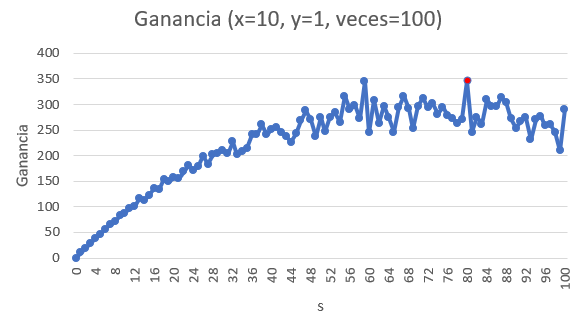
\includegraphics[width=100pt]{./graficas/10-1-100b.png}
			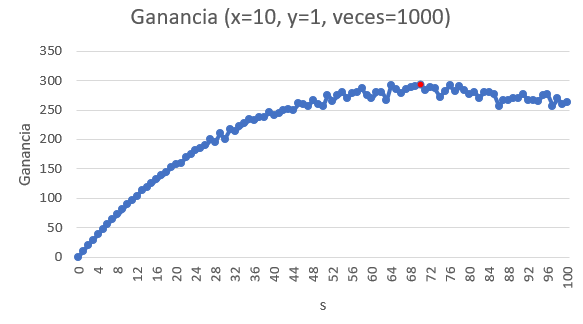
\includegraphics[width=100pt]{./graficas/10-1-1000b.png}
			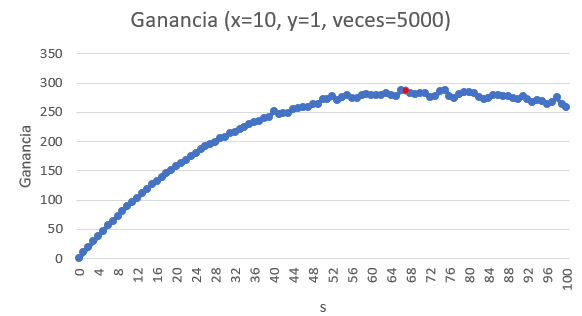
\includegraphics[width=100pt]{./graficas/10-1-5000b.png}
			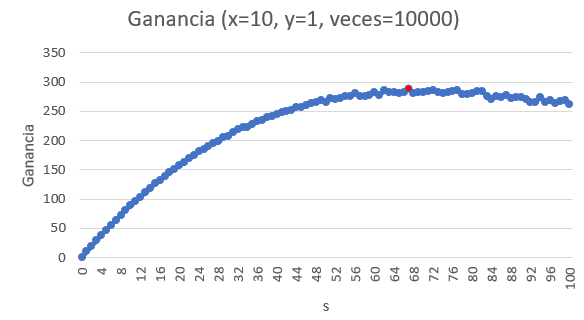
\includegraphics[width=100pt]{./graficas/10-1-10000b.png}
			\caption{Evolución de la Ganancia (x=10, y=1) Distribución B}
		\end{figure} 

	\newpage

	Como podemos ver la Figura 14 muestra la evolución de ganancia obtenida por cada valor 's' de las diferentes ejecuciones. Si observamos las gráficas donde el valor de 'veces' es superior a 1000 podemos ver como el valor de ganancia es creciente hasta que 's' tiene un valor próximo a 60, a partir de ese valor la ganancia se va equilibrando de forma moderada, también se puede apreciar como la ganancia empieza a decrecer al final de la ejecución. La gráfica con valor de veces=100 permite  ver como los valores obtenidos presentan una gran desviación. \\
	
	\begin{figure}[htb]
		\centering
		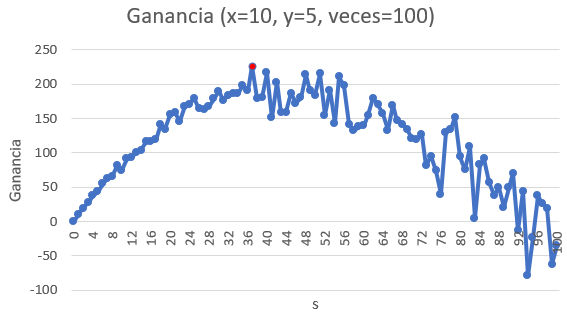
\includegraphics[width=150pt]{./graficas/10-5-100b.png}
		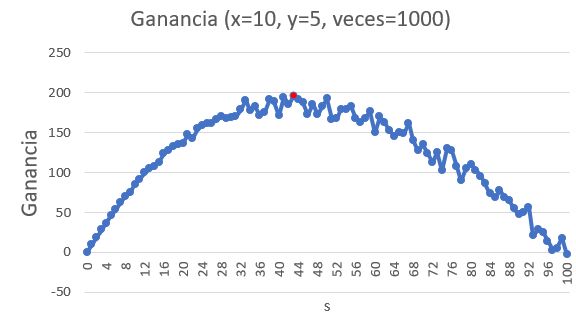
\includegraphics[width=150pt]{./graficas/10-5-1000b.png}
		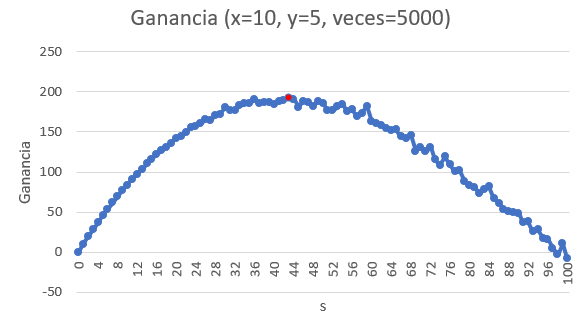
\includegraphics[width=150pt]{./graficas/10-5-5000b.png}
		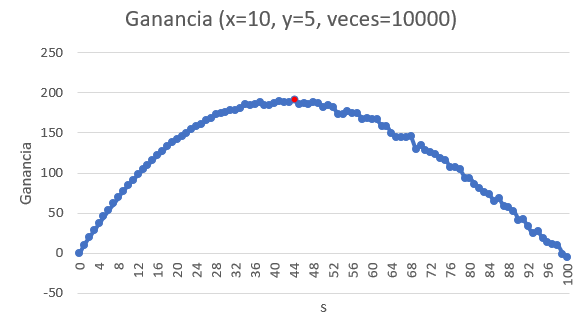
\includegraphics[width=150pt]{./graficas/10-5-10000b.png}
		\caption{Evolución de la Ganancia (x=10, y=5) Distribución B}
	\end{figure} 

	Mediante la observación de las gráficas obtenidas por esta distribución podemos decir que los valores son peores que los obtenidos en la distribución A. Vemos como los valores de 's' elevados causan una gran caída de la ganancia.
	
	
	\begin{figure}[h]
		\centering
		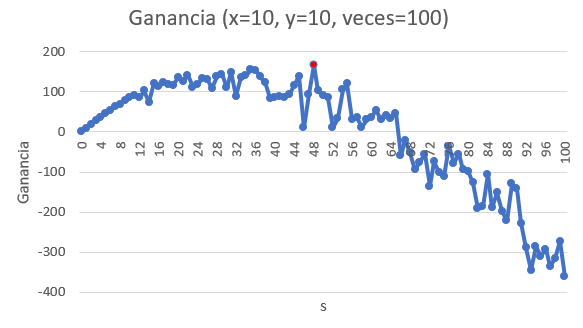
\includegraphics[width=100pt]{./graficas/10-10-100b.png}
		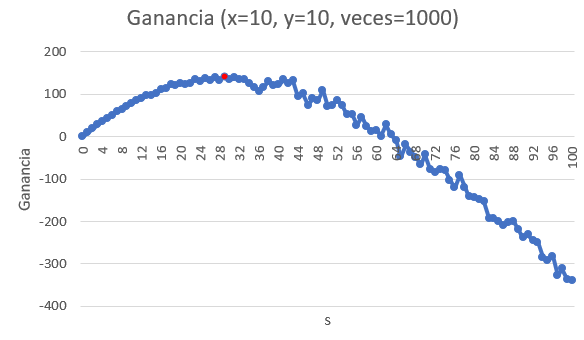
\includegraphics[width=100pt]{./graficas/10-10-1000b.png}
		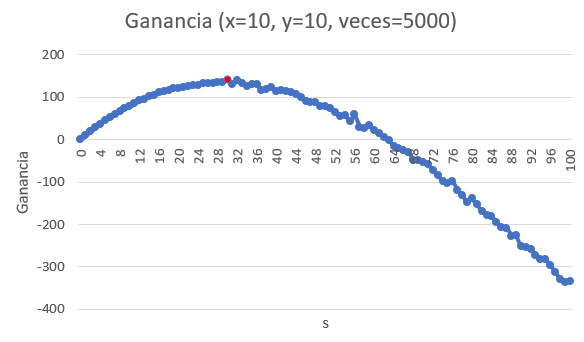
\includegraphics[width=100pt]{./graficas/10-10-5000b.png}
		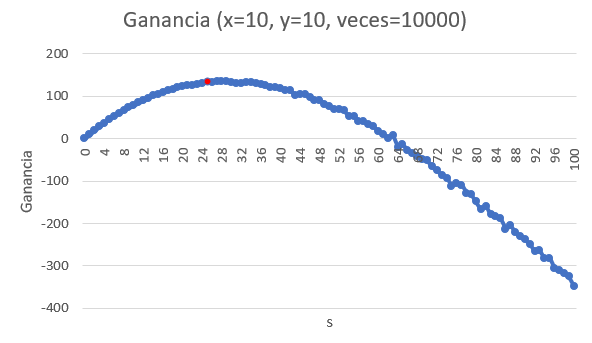
\includegraphics[width=100pt]{./graficas/10-10-10000b.png}
		\caption{Evolución de la Ganancia (x=10, y=10) Distribución B}
	\end{figure}


\begin{table}[h]
	\begin{tabular}{llllll}
		\hline
		\rowcolor[HTML]{F8A102} 
		\multicolumn{1}{|l|}{\cellcolor[HTML]{F8A102}{\color[HTML]{000000} x}} & \multicolumn{1}{l|}{\cellcolor[HTML]{F8A102}{\color[HTML]{000000} y}} & \multicolumn{1}{l|}{\cellcolor[HTML]{F8A102}{\color[HTML]{000000} veces}} & \multicolumn{1}{l|}{\cellcolor[HTML]{F8A102}{\color[HTML]{000000} Mejor\_s}} & \multicolumn{1}{l|}{\cellcolor[HTML]{F8A102}{\color[HTML]{000000} Mejor\_ganancia}} & \multicolumn{1}{l|}{\cellcolor[HTML]{F8A102}{\color[HTML]{000000} Mejor\_desviacion}} \\ \hline
		\multicolumn{1}{|l|}{}                                                 & \multicolumn{1}{l|}{}                                                 & \multicolumn{1}{l|}{100}                                                  & \multicolumn{1}{l|}{80}                                                      & \multicolumn{1}{l|}{346,58}                                                         & \multicolumn{1}{l|}{247,5504}                                                         \\ \cline{3-6} 
		\multicolumn{1}{|l|}{}                                                 & \multicolumn{1}{l|}{}                                                 & \multicolumn{1}{l|}{1000}                                                 & \multicolumn{1}{l|}{70}                                                      & \multicolumn{1}{l|}{293,396}                                                        & \multicolumn{1}{l|}{245,138}                                                          \\ \cline{3-6} 
		\multicolumn{1}{|l|}{}                                                 & \multicolumn{1}{l|}{}                                                 & \multicolumn{1}{l|}{5000}                                                 & \multicolumn{1}{l|}{67}                                                      & \multicolumn{1}{l|}{287,7874}                                                       & \multicolumn{1}{l|}{237,5177}                                                         \\ \cline{3-6} 
		\multicolumn{1}{|l|}{\multirow{-4}{*}{10}}                             & \multicolumn{1}{l|}{\multirow{-4}{*}{1}}                              & \multicolumn{1}{l|}{10000}                                                & \multicolumn{1}{l|}{67}                                                      & \multicolumn{1}{l|}{288,5904}                                                       & \multicolumn{1}{l|}{238,1739}                                                         \\ \hline
		&                                                                       &                                                                           &                                                                              &                                                                                     &                                                                                       \\ \hline
		\multicolumn{1}{|l|}{}                                                 & \multicolumn{1}{l|}{}                                                 & \multicolumn{1}{l|}{100}                                                  & \multicolumn{1}{l|}{37}                                                      & \multicolumn{1}{l|}{226,3}                                                          & \multicolumn{1}{l|}{177,2669}                                                         \\ \cline{3-6} 
		\multicolumn{1}{|l|}{}                                                 & \multicolumn{1}{l|}{}                                                 & \multicolumn{1}{l|}{1000}                                                 & \multicolumn{1}{l|}{43}                                                      & \multicolumn{1}{l|}{196,885}                                                        & \multicolumn{1}{l|}{221,3657}                                                         \\ \cline{3-6} 
		\multicolumn{1}{|l|}{}                                                 & \multicolumn{1}{l|}{}                                                 & \multicolumn{1}{l|}{5000}                                                 & \multicolumn{1}{l|}{43}                                                      & \multicolumn{1}{l|}{192,586}                                                        & \multicolumn{1}{l|}{226,7948}                                                         \\ \cline{3-6} 
		\multicolumn{1}{|l|}{\multirow{-4}{*}{10}}                             & \multicolumn{1}{l|}{\multirow{-4}{*}{5}}                              & \multicolumn{1}{l|}{10000}                                                & \multicolumn{1}{l|}{44}                                                      & \multicolumn{1}{l|}{191,5025}                                                       & \multicolumn{1}{l|}{231,2614}                                                         \\ \hline
		&                                                                       &                                                                           &                                                                              &                                                                                     &                                                                                       \\ \hline
		\multicolumn{1}{|l|}{}                                                 & \multicolumn{1}{l|}{}                                                 & \multicolumn{1}{l|}{100}                                                  & \multicolumn{1}{l|}{48}                                                      & \multicolumn{1}{l|}{168,2}                                                          & \multicolumn{1}{l|}{313,9207}                                                         \\ \cline{3-6} 
		\multicolumn{1}{|l|}{}                                                 & \multicolumn{1}{l|}{}                                                 & \multicolumn{1}{l|}{1000}                                                 & \multicolumn{1}{l|}{29}                                                      & \multicolumn{1}{l|}{142,68}                                                         & \multicolumn{1}{l|}{192,9239}                                                         \\ \cline{3-6} 
		\multicolumn{1}{|l|}{}                                                 & \multicolumn{1}{l|}{}                                                 & \multicolumn{1}{l|}{5000}                                                 & \multicolumn{1}{l|}{30}                                                      & \multicolumn{1}{l|}{141,312}                                                        & \multicolumn{1}{l|}{201,8927}                                                         \\ \cline{3-6} 
		\multicolumn{1}{|l|}{\multirow{-4}{*}{10}}                             & \multicolumn{1}{l|}{\multirow{-4}{*}{10}}                             & \multicolumn{1}{l|}{10000}                                                & \multicolumn{1}{l|}{25}                                                      & \multicolumn{1}{l|}{135,572}                                                        & \multicolumn{1}{l|}{162,8307}                                                         \\ \hline
	\end{tabular}
	\caption{Resultados Distribución B}
\end{table}

\newpage
	
Por otro lado, en la Tabla 2 vemos los mejores resultados obtenidos en las ejecuciones de la distribución B. Dos de las ejecuciones obtienen el valor s=67 como el mejor valor, las cuales son las ejecuciones con valor de veces=5000 y veces=100000, mientras que el resto de ejecuciones obtienen s=80 y s=70. Las desviaciones son similares entre los resultados. Si comparamos las ganancias, la mejor es obtenida por el valor veces=100 lo cual podría llevarnos a errores, ya que es mejor realizar cálculos para un largo periodo de tiempo ya que permitirá realizar un mejor balance sobre nuestras ganancias finales. \\

\newpage



\section*{c) - Distribución C (Distribución "triangular")}	
	En este apartado vamos a realizar los mismos experimentos que para las distribuciones anteriores. Esta distribución es triangular, es decir, para un rango de valores de 'd' la función de probabilidad es diferente al segundo rango de valores. 
	
		$$
		P(D=d)=\left\{\begin{array}{ll}{\frac{d}{2500}} & { { si } 0 \leq d<50} \\ {\frac{100-d}{2500}} & { { si } 50 \leq d \leq 99}\end{array}\right.
		$$
	
	\begin{figure}[h]
		\centering
		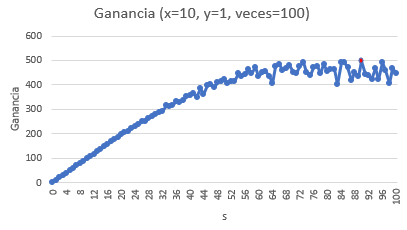
\includegraphics[width=150pt]{./graficas/10-1-100c.png}
		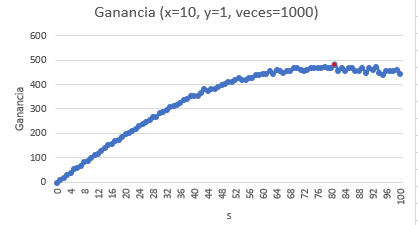
\includegraphics[width=150pt]{./graficas/10-1-1000c.png}
		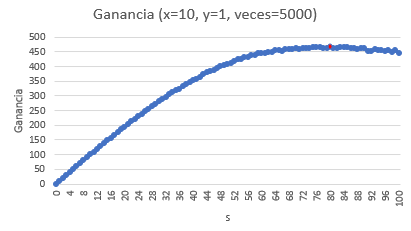
\includegraphics[width=150pt]{./graficas/10-1-5000c.png}
		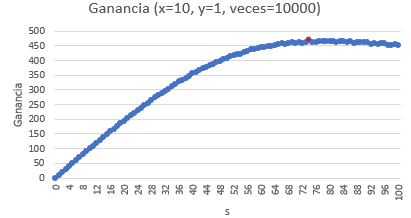
\includegraphics[width=150pt]{./graficas/10-1-10000c.png}
		\caption{Evolución de la Ganancia (x=10, y=1) Distribución C}
	\end{figure} 


	Mediante la Figura 7 vemos como el valor de ganancia crece considerablemente hasta llegar a un cierto valor de 's' donde a partir de ese valor la ganancia empieza a tomar valores equilibrados. Esto se debe a que llegamos a un cierto rango de 's' donde la ganancia experimenta poca variación entre esos valores.
	
	\begin{figure}[h]
		\centering
		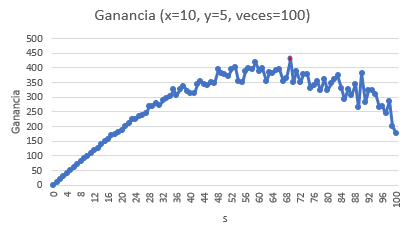
\includegraphics[width=100pt]{./graficas/10-5-100c.png}
		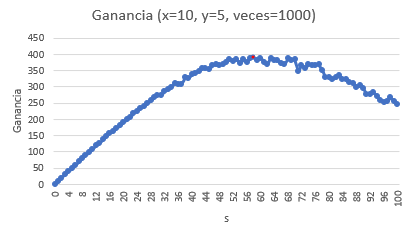
\includegraphics[width=100pt]{./graficas/10-5-1000c.png}
		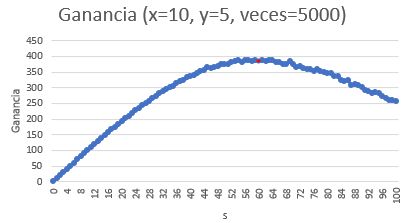
\includegraphics[width=100pt]{./graficas/10-5-5000c.png}
		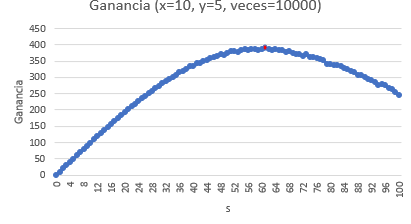
\includegraphics[width=100pt]{./graficas/10-5-10000c.png}
		\caption{Evolución de la Ganancia (x=10, y=5) Distribución C}
	\end{figure} 
	\newpage
	
	Cuando el valor de perdida es incrementado vemos como la ganancia decae cuando aumentados el valor de 's'. También se puede apreciar como el valor de veces ejerce una gran variación entre los valores de ganancia, es decir, cuando veces es pequeño vemos como la evolución de la ganancia tiene muchos picos altos y bajos, en cambio para valores de veces mayor estos picos disminuyen.
	
	
	\begin{figure}[h]
		\centering
		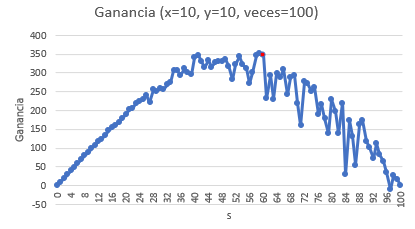
\includegraphics[width=100pt]{./graficas/10-10-100c.png}
		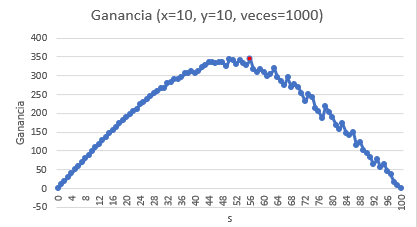
\includegraphics[width=100pt]{./graficas/10-10-1000c.png}
		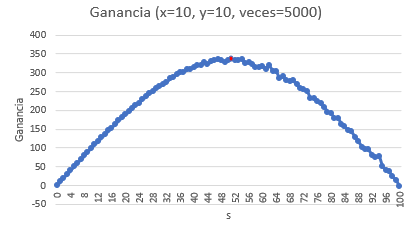
\includegraphics[width=100pt]{./graficas/10-10-5000c.png}
		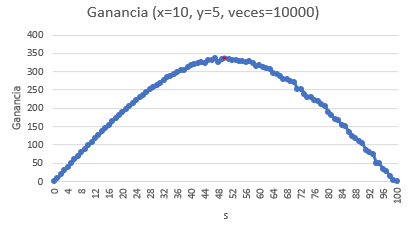
\includegraphics[width=100pt]{./graficas/10-10-10000c.png}
		\caption{Evolución de la Ganancia (x=10, y=10) Distribución C}
	\end{figure} 

	Para finalizar este apartado, vamos a analizar los resultados obtenidos en las diferentes ejecuciones. En la tabla 3 vemos los mejores resultados obtenidos en cada ejecución, como hemos visto en los resultados de las distribuciones anteriores cuando el valor de perdido es mayor el valor de 's' disminuye al igual que la ganancia, en cambio en esta distribución vemos como los valores de desviación son similares entre las ejecuciones de los diferentes parámetros.


	\begin{table}[h]
		\begin{tabular}{llllll}
			\hline
			\rowcolor[HTML]{F8A102} 
			\multicolumn{1}{|l|}{\cellcolor[HTML]{F8A102}{\color[HTML]{000000} x}} & \multicolumn{1}{l|}{\cellcolor[HTML]{F8A102}{\color[HTML]{000000} y}} & \multicolumn{1}{l|}{\cellcolor[HTML]{F8A102}{\color[HTML]{000000} veces}} & \multicolumn{1}{l|}{\cellcolor[HTML]{F8A102}{\color[HTML]{000000} Mejor\_s}} & \multicolumn{1}{l|}{\cellcolor[HTML]{F8A102}{\color[HTML]{000000} Mejor\_ganancia}} & \multicolumn{1}{l|}{\cellcolor[HTML]{F8A102}{\color[HTML]{000000} Mejor\_desviacion}} \\ \hline
			\multicolumn{1}{|l|}{}                                                 & \multicolumn{1}{l|}{}                                                 & \multicolumn{1}{l|}{100}                                                  & \multicolumn{1}{l|}{90}                                                      & \multicolumn{1}{l|}{494,32}                                                         & \multicolumn{1}{l|}{225,3531}                                                         \\ \cline{3-6} 
			\multicolumn{1}{|l|}{}                                                 & \multicolumn{1}{l|}{}                                                 & \multicolumn{1}{l|}{1000}                                                 & \multicolumn{1}{l|}{81}                                                      & \multicolumn{1}{l|}{476,414}                                                        & \multicolumn{1}{l|}{215,3639}                                                         \\ \cline{3-6} 
			\multicolumn{1}{|l|}{}                                                 & \multicolumn{1}{l|}{}                                                 & \multicolumn{1}{l|}{5000}                                                 & \multicolumn{1}{l|}{80}                                                      & \multicolumn{1}{l|}{466,3854}                                                       & \multicolumn{1}{l|}{210,0757}                                                         \\ \cline{3-6} 
			\multicolumn{1}{|l|}{\multirow{-4}{*}{10}}                             & \multicolumn{1}{l|}{\multirow{-4}{*}{1}}                              & \multicolumn{1}{l|}{10000}                                                & \multicolumn{1}{l|}{74}                                                      & \multicolumn{1}{l|}{467,7874}                                                       & \multicolumn{1}{l|}{204,1891}                                                         \\ \hline
			&                                                                       &                                                                           &                                                                              &                                                                                     &                                                                                       \\ \hline
			\multicolumn{1}{|l|}{}                                                 & \multicolumn{1}{l|}{}                                                 & \multicolumn{1}{l|}{100}                                                  & \multicolumn{1}{l|}{69}                                                      & \multicolumn{1}{l|}{429,15}                                                         & \multicolumn{1}{l|}{264,5742}                                                         \\ \cline{3-6} 
			\multicolumn{1}{|l|}{}                                                 & \multicolumn{1}{l|}{}                                                 & \multicolumn{1}{l|}{1000}                                                 & \multicolumn{1}{l|}{58}                                                      & \multicolumn{1}{l|}{392,29}                                                         & \multicolumn{1}{l|}{221,0417}                                                         \\ \cline{3-6} 
			\multicolumn{1}{|l|}{}                                                 & \multicolumn{1}{l|}{}                                                 & \multicolumn{1}{l|}{5000}                                                 & \multicolumn{1}{l|}{59}                                                      & \multicolumn{1}{l|}{387,965}                                                        & \multicolumn{1}{l|}{222,0404}                                                         \\ \cline{3-6} 
			\multicolumn{1}{|l|}{\multirow{-4}{*}{10}}                             & \multicolumn{1}{l|}{\multirow{-4}{*}{5}}                              & \multicolumn{1}{l|}{10000}                                                & \multicolumn{1}{l|}{61}                                                      & \multicolumn{1}{l|}{389,9275}                                                       & \multicolumn{1}{l|}{227,0186}                                                         \\ \hline
			&                                                                       &                                                                           &                                                                              &                                                                                     &                                                                                       \\ \hline
			\multicolumn{1}{|l|}{}                                                 & \multicolumn{1}{l|}{}                                                 & \multicolumn{1}{l|}{100}                                                  & \multicolumn{1}{l|}{59}                                                      & \multicolumn{1}{l|}{351,8}                                                          & \multicolumn{1}{l|}{295,5713}                                                         \\ \cline{3-6} 
			\multicolumn{1}{|l|}{}                                                 & \multicolumn{1}{l|}{}                                                 & \multicolumn{1}{l|}{1000}                                                 & \multicolumn{1}{l|}{56}                                                      & \multicolumn{1}{l|}{343,78}                                                         & \multicolumn{1}{l|}{263,3892}                                                         \\ \cline{3-6} 
			\multicolumn{1}{|l|}{}                                                 & \multicolumn{1}{l|}{}                                                 & \multicolumn{1}{l|}{5000}                                                 & \multicolumn{1}{l|}{51}                                                      & \multicolumn{1}{l|}{336,568}                                                        & \multicolumn{1}{l|}{242,6352}                                                         \\ \cline{3-6} 
			\multicolumn{1}{|l|}{\multirow{-4}{*}{10}}                             & \multicolumn{1}{l|}{\multirow{-4}{*}{10}}                             & \multicolumn{1}{l|}{10000}                                                & \multicolumn{1}{l|}{50}                                                      & \multicolumn{1}{l|}{335,688}                                                        & \multicolumn{1}{l|}{235,6051}                                                         \\ \hline
		\end{tabular}
	\caption{Resultados Distribución C}
	\end{table}
	
	\newpage


	\Large \textbf{1.2) - Modificaciones del Modelo} \\
	
	\normalsize En este apartado vamos a realizar modificaciones sobre la manera de enfocar las perdidas cuando no se consiguen vender todos los productos. \\
	
	
	\normalsize \textbf{1.2.1) Modificación 1 (costo de perdida fijo 'z')} \\
	
	La primera modificación consiste en fijar un valor 'z', el cual será la cantidad a pagar cuando los productos diarias no son vendidos por completo. Esto supone que por cada producto que no vendemos no paguemos ninguna cantidad de perdida, ya que para cualquier cantidad no vendida la perdida va a ser el valor 'z'. \\
	
	Vamos a realizar pruebas de esta modificación sobre las distintas distribuciones y parámetros comentados en apartados anteriores. El valor de 'z' varia entre 10, 50 y 100 para todas las distribuciones. \\
	

	\textbf{-Distribución A-}

	\begin{table}[h]
		\begin{tabular}{llllll}
			\hline
			\rowcolor[HTML]{F8A102} 
			\multicolumn{1}{|l|}{\cellcolor[HTML]{F8A102}{\color[HTML]{000000} x}} & \multicolumn{1}{l|}{\cellcolor[HTML]{F8A102}{\color[HTML]{000000} z}} & \multicolumn{1}{l|}{\cellcolor[HTML]{F8A102}{\color[HTML]{000000} veces}} & \multicolumn{1}{l|}{\cellcolor[HTML]{F8A102}{\color[HTML]{000000} Mejor\_s}} & \multicolumn{1}{l|}{\cellcolor[HTML]{F8A102}{\color[HTML]{000000} Mejor\_ganancia}} & \multicolumn{1}{l|}{\cellcolor[HTML]{F8A102}{\color[HTML]{000000} Mejor\_desviacion}} \\ \hline
			\multicolumn{1}{|l|}{}                                                 & \multicolumn{1}{l|}{}                                                 & \multicolumn{1}{l|}{100}                                                  & \multicolumn{1}{l|}{90}                                                      & \multicolumn{1}{l|}{550,70}                                                         & \multicolumn{1}{l|}{2621,79}                                                          \\ \cline{3-6} 
			\multicolumn{1}{|l|}{}                                                 & \multicolumn{1}{l|}{}                                                 & \multicolumn{1}{l|}{1000}                                                 & \multicolumn{1}{l|}{100}                                                     & \multicolumn{1}{l|}{494,00}                                                         & \multicolumn{1}{l|}{282,22}                                                           \\ \cline{3-6} 
			\multicolumn{1}{|l|}{}                                                 & \multicolumn{1}{l|}{}                                                 & \multicolumn{1}{l|}{5000}                                                 & \multicolumn{1}{l|}{99}                                                      & \multicolumn{1}{l|}{491,83}                                                         & \multicolumn{1}{l|}{286,35}                                                           \\ \cline{3-6} 
			\multicolumn{1}{|l|}{\multirow{-4}{*}{10}}                             & \multicolumn{1}{l|}{\multirow{-4}{*}{10}}                             & \multicolumn{1}{l|}{10000}                                                & \multicolumn{1}{l|}{99}                                                      & \multicolumn{1}{l|}{491,95}                                                         & \multicolumn{1}{l|}{288,98}                                                           \\ \hline
			&                                                                       &                                                                           &                                                                              &                                                                                     &                                                                                       \\ \hline
			\multicolumn{1}{|l|}{}                                                 & \multicolumn{1}{l|}{}                                                 & \multicolumn{1}{l|}{100}                                                  & \multicolumn{1}{l|}{94}                                                      & \multicolumn{1}{l|}{497,70}                                                         & \multicolumn{1}{l|}{293,80}                                                           \\ \cline{3-6} 
			\multicolumn{1}{|l|}{}                                                 & \multicolumn{1}{l|}{}                                                 & \multicolumn{1}{l|}{1000}                                                 & \multicolumn{1}{l|}{91}                                                      & \multicolumn{1}{l|}{458,26}                                                         & \multicolumn{1}{l|}{289,50}                                                           \\ \cline{3-6} 
			\multicolumn{1}{|l|}{}                                                 & \multicolumn{1}{l|}{}                                                 & \multicolumn{1}{l|}{5000}                                                 & \multicolumn{1}{l|}{96}                                                      & \multicolumn{1}{l|}{453,82}                                                         & \multicolumn{1}{l|}{290,92}                                                           \\ \cline{3-6} 
			\multicolumn{1}{|l|}{\multirow{-4}{*}{10}}                             & \multicolumn{1}{l|}{\multirow{-4}{*}{50}}                             & \multicolumn{1}{l|}{10000}                                                & \multicolumn{1}{l|}{100}                                                     & \multicolumn{1}{l|}{449,28}                                                         & \multicolumn{1}{l|}{288,51}                                                           \\ \hline
			&                                                                       &                                                                           &                                                                              &                                                                                     &                                                                                       \\ \hline
			\multicolumn{1}{|l|}{}                                                 & \multicolumn{1}{l|}{}                                                 & \multicolumn{1}{l|}{100}                                                  & \multicolumn{1}{l|}{91}                                                      & \multicolumn{1}{l|}{459,00}                                                         & \multicolumn{1}{l|}{309,04}                                                           \\ \cline{3-6} 
			\multicolumn{1}{|l|}{}                                                 & \multicolumn{1}{l|}{}                                                 & \multicolumn{1}{l|}{1000}                                                 & \multicolumn{1}{l|}{97}                                                      & \multicolumn{1}{l|}{409,05}                                                         & \multicolumn{1}{l|}{288,00}                                                           \\ \cline{3-6} 
			\multicolumn{1}{|l|}{}                                                 & \multicolumn{1}{l|}{}                                                 & \multicolumn{1}{l|}{5000}                                                 & \multicolumn{1}{l|}{85}                                                      & \multicolumn{1}{l|}{407,04}                                                         & \multicolumn{1}{l|}{295,93}                                                           \\ \cline{3-6} 
			\multicolumn{1}{|l|}{\multirow{-4}{*}{10}}                             & \multicolumn{1}{l|}{\multirow{-4}{*}{100}}                            & \multicolumn{1}{l|}{10000}                                                & \multicolumn{1}{l|}{86}                                                      & \multicolumn{1}{l|}{404,87}                                                         & \multicolumn{1}{l|}{294,42}                                                           \\ \hline
		\end{tabular}
	\caption{Resultado Distribución A (Modificación 1)}
	\end{table}

	Observando la Tabla 4, podemos ver como el valor de 's' obtenido como mejor es alto esto se debe a que la perdida por no vender todos los productos no es muy alta, lo cual permite pedir una mayor cantidad de productos ya que la ganancia aumentará mas rápido que perdidas se producen. 

	\newpage

	\textbf{-Distribución B-} \\
	
	Esta distribución obtiene en media un valor de 's' más bajo que la primera distribución (aunque la diferencia no es elevada). Por consecuencia, el valor de ganancia obtenido es mas baja que la anterior esto se debe a que la frecuencia de perdida es mayor.
	

	\begin{table}[h]
		\begin{tabular}{llllll}
			\hline
			\rowcolor[HTML]{F8A102} 
			\multicolumn{1}{|l|}{\cellcolor[HTML]{F8A102}{\color[HTML]{000000} x}} & \multicolumn{1}{l|}{\cellcolor[HTML]{F8A102}{\color[HTML]{000000} z}} & \multicolumn{1}{l|}{\cellcolor[HTML]{F8A102}{\color[HTML]{000000} veces}} & \multicolumn{1}{l|}{\cellcolor[HTML]{F8A102}{\color[HTML]{000000} Mejor\_s}} & \multicolumn{1}{l|}{\cellcolor[HTML]{F8A102}{\color[HTML]{000000} Mejor\_ganancia}} & \multicolumn{1}{l|}{\cellcolor[HTML]{F8A102}{\color[HTML]{000000} Mejor\_desviacion}} \\ \hline
			\multicolumn{1}{|l|}{}                                                 & \multicolumn{1}{l|}{}                                                 & \multicolumn{1}{l|}{100}                                                  & \multicolumn{1}{l|}{97}                                                      & \multicolumn{1}{l|}{369,40}                                                         & \multicolumn{1}{l|}{252,41}                                                           \\ \cline{3-6} 
			\multicolumn{1}{|l|}{}                                                 & \multicolumn{1}{l|}{}                                                 & \multicolumn{1}{l|}{1000}                                                 & \multicolumn{1}{l|}{78}                                                      & \multicolumn{1}{l|}{332,39}                                                         & \multicolumn{1}{l|}{232,50}                                                           \\ \cline{3-6} 
			\multicolumn{1}{|l|}{}                                                 & \multicolumn{1}{l|}{}                                                 & \multicolumn{1}{l|}{5000}                                                 & \multicolumn{1}{l|}{97}                                                      & \multicolumn{1}{l|}{326,64}                                                         & \multicolumn{1}{l|}{238,79}                                                           \\ \cline{3-6} 
			\multicolumn{1}{|l|}{\multirow{-4}{*}{10}}                             & \multicolumn{1}{l|}{\multirow{-4}{*}{10}}                             & \multicolumn{1}{l|}{10000}                                                & \multicolumn{1}{l|}{90}                                                      & \multicolumn{1}{l|}{324,80}                                                         & \multicolumn{1}{l|}{238,08}                                                           \\ \hline
			&                                                                       &                                                                           &                                                                              &                                                                                     &                                                                                       \\ \hline
			\multicolumn{1}{|l|}{}                                                 & \multicolumn{1}{l|}{}                                                 & \multicolumn{1}{l|}{100}                                                  & \multicolumn{1}{l|}{75}                                                      & \multicolumn{1}{l|}{325,70}                                                         & \multicolumn{1}{l|}{256,11}                                                           \\ \cline{3-6} 
			\multicolumn{1}{|l|}{}                                                 & \multicolumn{1}{l|}{}                                                 & \multicolumn{1}{l|}{1000}                                                 & \multicolumn{1}{l|}{92}                                                      & \multicolumn{1}{l|}{293,06}                                                         & \multicolumn{1}{l|}{237,59}                                                           \\ \cline{3-6} 
			\multicolumn{1}{|l|}{}                                                 & \multicolumn{1}{l|}{}                                                 & \multicolumn{1}{l|}{5000}                                                 & \multicolumn{1}{l|}{89}                                                      & \multicolumn{1}{l|}{284,35}                                                         & \multicolumn{1}{l|}{238,43}                                                           \\ \cline{3-6} 
			\multicolumn{1}{|l|}{\multirow{-4}{*}{10}}                             & \multicolumn{1}{l|}{\multirow{-4}{*}{50}}                             & \multicolumn{1}{l|}{10000}                                                & \multicolumn{1}{l|}{83}                                                      & \multicolumn{1}{l|}{287,95}                                                         & \multicolumn{1}{l|}{238,21}                                                           \\ \hline
			&                                                                       &                                                                           &                                                                              &                                                                                     &                                                                                       \\ \hline
			\multicolumn{1}{|l|}{}                                                 & \multicolumn{1}{l|}{}                                                 & \multicolumn{1}{l|}{100}                                                  & \multicolumn{1}{l|}{94}                                                      & \multicolumn{1}{l|}{272,20}                                                         & \multicolumn{1}{l|}{264,14}                                                           \\ \cline{3-6} 
			\multicolumn{1}{|l|}{}                                                 & \multicolumn{1}{l|}{}                                                 & \multicolumn{1}{l|}{1000}                                                 & \multicolumn{1}{l|}{88}                                                      & \multicolumn{1}{l|}{249,25}                                                         & \multicolumn{1}{l|}{246,00}                                                           \\ \cline{3-6} 
			\multicolumn{1}{|l|}{}                                                 & \multicolumn{1}{l|}{}                                                 & \multicolumn{1}{l|}{5000}                                                 & \multicolumn{1}{l|}{92}                                                      & \multicolumn{1}{l|}{238,96}                                                         & \multicolumn{1}{l|}{243,17}                                                           \\ \cline{3-6} 
			\multicolumn{1}{|l|}{\multirow{-4}{*}{10}}                             & \multicolumn{1}{l|}{\multirow{-4}{*}{100}}                            & \multicolumn{1}{l|}{10000}                                                & \multicolumn{1}{l|}{87}                                                      & \multicolumn{1}{l|}{235,36}                                                         & \multicolumn{1}{l|}{238,91}                                                           \\ \hline
		\end{tabular}
	\caption{Resultado Distribución B (Modificación 1)}
	\end{table} 

	\vspace{1cm}

	\textbf{-Distribución C-} \\
	
	Por último, observando la Tabla 6 vemos como los resultados en cuanto respecta al valor de 's' es muy parecido a la distribución B del apartado anterior, pero la ganancia es mucho mayor que la anterior.
	
	\newpage
	
	\begin{table}[h]
		\begin{tabular}{llllll}
			\hline
			\rowcolor[HTML]{F8A102} 
			\multicolumn{1}{|l|}{\cellcolor[HTML]{F8A102}{\color[HTML]{000000} x}} & \multicolumn{1}{l|}{\cellcolor[HTML]{F8A102}{\color[HTML]{000000} z}} & \multicolumn{1}{l|}{\cellcolor[HTML]{F8A102}{\color[HTML]{000000} veces}} & \multicolumn{1}{l|}{\cellcolor[HTML]{F8A102}{\color[HTML]{000000} Mejor\_s}} & \multicolumn{1}{l|}{\cellcolor[HTML]{F8A102}{\color[HTML]{000000} Mejor\_ganancia}} & \multicolumn{1}{l|}{\cellcolor[HTML]{F8A102}{\color[HTML]{000000} Mejor\_desviacion}} \\ \hline
			\multicolumn{1}{|l|}{}                                                 & \multicolumn{1}{l|}{}                                                 & \multicolumn{1}{l|}{100}                                                  & \multicolumn{1}{l|}{93}                                                      & \multicolumn{1}{l|}{520,80}                                                         & \multicolumn{1}{l|}{197,75}                                                           \\ \cline{3-6} 
			\multicolumn{1}{|l|}{}                                                 & \multicolumn{1}{l|}{}                                                 & \multicolumn{1}{l|}{1000}                                                 & \multicolumn{1}{l|}{80}                                                      & \multicolumn{1}{l|}{504,10}                                                         & \multicolumn{1}{l|}{196,08}                                                           \\ \cline{3-6} 
			\multicolumn{1}{|l|}{}                                                 & \multicolumn{1}{l|}{}                                                 & \multicolumn{1}{l|}{5000}                                                 & \multicolumn{1}{l|}{91}                                                      & \multicolumn{1}{l|}{496,92}                                                         & \multicolumn{1}{l|}{201,94}                                                           \\ \cline{3-6} 
			\multicolumn{1}{|l|}{\multirow{-4}{*}{10}}                             & \multicolumn{1}{l|}{\multirow{-4}{*}{10}}                             & \multicolumn{1}{l|}{10000}                                                & \multicolumn{1}{l|}{86}                                                      & \multicolumn{1}{l|}{492,63}                                                         & \multicolumn{1}{l|}{199,95}                                                           \\ \hline
			&                                                                       &                                                                           &                                                                              &                                                                                     &                                                                                       \\ \hline
			\multicolumn{1}{|l|}{}                                                 & \multicolumn{1}{l|}{}                                                 & \multicolumn{1}{l|}{100}                                                  & \multicolumn{1}{l|}{75}                                                      & \multicolumn{1}{l|}{482,00}                                                         & \multicolumn{1}{l|}{190,28}                                                           \\ \cline{3-6} 
			\multicolumn{1}{|l|}{}                                                 & \multicolumn{1}{l|}{}                                                 & \multicolumn{1}{l|}{1000}                                                 & \multicolumn{1}{l|}{86}                                                      & \multicolumn{1}{l|}{466,67}                                                         & \multicolumn{1}{l|}{210,70}                                                           \\ \cline{3-6} 
			\multicolumn{1}{|l|}{}                                                 & \multicolumn{1}{l|}{}                                                 & \multicolumn{1}{l|}{5000}                                                 & \multicolumn{1}{l|}{85}                                                      & \multicolumn{1}{l|}{455,90}                                                         & \multicolumn{1}{l|}{205,73}                                                           \\ \cline{3-6} 
			\multicolumn{1}{|l|}{\multirow{-4}{*}{10}}                             & \multicolumn{1}{l|}{\multirow{-4}{*}{50}}                             & \multicolumn{1}{l|}{10000}                                                & \multicolumn{1}{l|}{94}                                                      & \multicolumn{1}{l|}{454,48}                                                         & \multicolumn{1}{l|}{204,37}                                                           \\ \hline
			&                                                                       &                                                                           &                                                                              &                                                                                     &                                                                                       \\ \hline
			\multicolumn{1}{|l|}{}                                                 & \multicolumn{1}{l|}{}                                                 & \multicolumn{1}{l|}{100}                                                  & \multicolumn{1}{l|}{92}                                                      & \multicolumn{1}{l|}{458,30}                                                         & \multicolumn{1}{l|}{217,26}                                                           \\ \cline{3-6} 
			\multicolumn{1}{|l|}{}                                                 & \multicolumn{1}{l|}{}                                                 & \multicolumn{1}{l|}{1000}                                                 & \multicolumn{1}{l|}{88}                                                      & \multicolumn{1}{l|}{409,48}                                                         & \multicolumn{1}{l|}{212,08}                                                           \\ \cline{3-6} 
			\multicolumn{1}{|l|}{}                                                 & \multicolumn{1}{l|}{}                                                 & \multicolumn{1}{l|}{5000}                                                 & \multicolumn{1}{l|}{80}                                                      & \multicolumn{1}{l|}{409,98}                                                         & \multicolumn{1}{l|}{214,00}                                                           \\ \cline{3-6} 
			\multicolumn{1}{|l|}{\multirow{-4}{*}{10}}                             & \multicolumn{1}{l|}{\multirow{-4}{*}{100}}                            & \multicolumn{1}{l|}{10000}                                                & \multicolumn{1}{l|}{78}                                                      & \multicolumn{1}{l|}{406,63}                                                         & \multicolumn{1}{l|}{211,81}                                                           \\ \hline
		\end{tabular}
		\caption{Resultado Distribución C (Modificación 1)}
	\end{table}

	\vspace{1cm}

	\underline{\textbf{Conclusión}} \\
	
	 En conclusión, esta primera modificación obtiene mejores resultados que el programa original. Esto puede deberse al mejor rendimiento en la perdida de ganancia por los productos no vendidos. La ganancia conseguida por las diferentes ejecuciones mejora con respecto al original. Tenemos que destacar que no siempre será mejor esta opción ya que si todos los días no vendemos 3 productos y cada uno tiene una perdida de 1 euro, sería mas eficiente pagar 1 euro por cada producto que pagar una cuantía fija que puede ser mayor que esta cantidad, esto es lo más común en este tipo de contratos.



\newpage
	
	\normalsize \textbf{1.2.2) Modificación 2 (perdida = $x * d-\min \{z,(s-d) * y\}$)} \\
	
	En este experimento, tras la conclusión de la sección anterior, vamos a mejorar el rendimiento de las perdidas. Como hemos dicho antes no es lo mismo pagar 1 euro * 3 productos que una cuantía fija de 30 euros, por lo cual esta modificación consiste en seleccionar el mínimo valor entre dicha cuantía fija 'z' y el costo total de la suma de las perdidas de cada producto. \\
	
	\textbf{-Distribución A-} \\
	
	Comenzamos con las pruebas sobre la distribución A, como observamos en la Tabla 7 las diferencias en las ganancias mejoran un poco respecto a la modificación 1 y el programa original. La desviación es similar en ambas modificaciones.
	
	
	\begin{table}[h]
		\begin{tabular}{lllllll}
			\hline
			\rowcolor[HTML]{F8A102} 
			\multicolumn{1}{|l|}{\cellcolor[HTML]{F8A102}{\color[HTML]{000000} x}} & \multicolumn{1}{l|}{\cellcolor[HTML]{F8A102}y} & \multicolumn{1}{l|}{\cellcolor[HTML]{F8A102}{\color[HTML]{000000} z}} & \multicolumn{1}{l|}{\cellcolor[HTML]{F8A102}{\color[HTML]{000000} veces}} & \multicolumn{1}{l|}{\cellcolor[HTML]{F8A102}{\color[HTML]{000000} Mejor\_s}} & \multicolumn{1}{l|}{\cellcolor[HTML]{F8A102}{\color[HTML]{000000} Mejor\_ganancia}} & \multicolumn{1}{l|}{\cellcolor[HTML]{F8A102}{\color[HTML]{000000} Mejor\_desviacion}} \\ \hline
			\multicolumn{1}{|l|}{}                                                 & \multicolumn{1}{l|}{}                          & \multicolumn{1}{l|}{}                                                 & \multicolumn{1}{l|}{100}                                                  & \multicolumn{1}{l|}{92}                                                      & \multicolumn{1}{l|}{540,54}                                                         & \multicolumn{1}{l|}{259,77}                                                           \\ \cline{4-7} 
			\multicolumn{1}{|l|}{}                                                 & \multicolumn{1}{l|}{}                          & \multicolumn{1}{l|}{}                                                 & \multicolumn{1}{l|}{1000}                                                 & \multicolumn{1}{l|}{93}                                                      & \multicolumn{1}{l|}{502,55}                                                         & \multicolumn{1}{l|}{286,81}                                                           \\ \cline{4-7} 
			\multicolumn{1}{|l|}{}                                                 & \multicolumn{1}{l|}{}                          & \multicolumn{1}{l|}{}                                                 & \multicolumn{1}{l|}{5000}                                                 & \multicolumn{1}{l|}{94}                                                      & \multicolumn{1}{l|}{491,89}                                                         & \multicolumn{1}{l|}{286,53}                                                           \\ \cline{4-7} 
			\multicolumn{1}{|l|}{\multirow{-4}{*}{10}}                             & \multicolumn{1}{l|}{\multirow{-4}{*}{1}}       & \multicolumn{1}{l|}{\multirow{-4}{*}{10}}                             & \multicolumn{1}{l|}{10000}                                                & \multicolumn{1}{l|}{95}                                                      & \multicolumn{1}{l|}{487,44}                                                         & \multicolumn{1}{l|}{288,91}                                                           \\ \hline
			&                                                &                                                                       &                                                                           &                                                                              &                                                                                     &                                                                                       \\ \hline
			\multicolumn{1}{|l|}{}                                                 & \multicolumn{1}{l|}{}                          & \multicolumn{1}{l|}{}                                                 & \multicolumn{1}{l|}{100}                                                  & \multicolumn{1}{l|}{95}                                                      & \multicolumn{1}{l|}{513,05}                                                         & \multicolumn{1}{l|}{326,85}                                                           \\ \cline{4-7} 
			\multicolumn{1}{|l|}{}                                                 & \multicolumn{1}{l|}{}                          & \multicolumn{1}{l|}{}                                                 & \multicolumn{1}{l|}{1000}                                                 & \multicolumn{1}{l|}{86}                                                      & \multicolumn{1}{l|}{461,83}                                                         & \multicolumn{1}{l|}{286,85}                                                           \\ \cline{4-7} 
			\multicolumn{1}{|l|}{}                                                 & \multicolumn{1}{l|}{}                          & \multicolumn{1}{l|}{}                                                 & \multicolumn{1}{l|}{5000}                                                 & \multicolumn{1}{l|}{94}                                                      & \multicolumn{1}{l|}{457,71}                                                         & \multicolumn{1}{l|}{294,42}                                                           \\ \cline{4-7} 
			\multicolumn{1}{|l|}{\multirow{-4}{*}{10}}                             & \multicolumn{1}{l|}{\multirow{-4}{*}{5}}       & \multicolumn{1}{l|}{\multirow{-4}{*}{50}}                             & \multicolumn{1}{l|}{10000}                                                & \multicolumn{1}{l|}{94}                                                      & \multicolumn{1}{l|}{452,60}                                                         & \multicolumn{1}{l|}{294,56}                                                           \\ \hline
			&                                                &                                                                       &                                                                           &                                                                              &                                                                                     &                                                                                       \\ \hline
			\multicolumn{1}{|l|}{}                                                 & \multicolumn{1}{l|}{}                          & \multicolumn{1}{l|}{}                                                 & \multicolumn{1}{l|}{100}                                                  & \multicolumn{1}{l|}{79}                                                      & \multicolumn{1}{l|}{458,10}                                                         & \multicolumn{1}{l|}{295,17}                                                           \\ \cline{4-7} 
			\multicolumn{1}{|l|}{}                                                 & \multicolumn{1}{l|}{}                          & \multicolumn{1}{l|}{}                                                 & \multicolumn{1}{l|}{1000}                                                 & \multicolumn{1}{l|}{95}                                                      & \multicolumn{1}{l|}{416,62}                                                         & \multicolumn{1}{l|}{296,94}                                                           \\ \cline{4-7} 
			\multicolumn{1}{|l|}{}                                                 & \multicolumn{1}{l|}{}                          & \multicolumn{1}{l|}{}                                                 & \multicolumn{1}{l|}{5000}                                                 & \multicolumn{1}{l|}{88}                                                      & \multicolumn{1}{l|}{412,65}                                                         & \multicolumn{1}{l|}{299,72}                                                           \\ \cline{4-7} 
			\multicolumn{1}{|l|}{\multirow{-4}{*}{10}}                             & \multicolumn{1}{l|}{\multirow{-4}{*}{10}}      & \multicolumn{1}{l|}{\multirow{-4}{*}{100}}                            & \multicolumn{1}{l|}{10000}                                                & \multicolumn{1}{l|}{85}                                                      & \multicolumn{1}{l|}{408,41}                                                         & \multicolumn{1}{l|}{300,69}                                                           \\ \hline
		\end{tabular}
	\caption{Resultado Distribución A (Modificación 2)}
	\end{table}

	\vspace{2cm}


	\textbf{-Distribución B-} \\
	
	De igual forma pasa con la distribución B, se puede ver una leve mejoría sobre los resultados en comparación con la modificación 1.
	
	\begin{table}[h]
		\begin{tabular}{lllllll}
			\hline
			\rowcolor[HTML]{F8A102} 
			\multicolumn{1}{|l|}{\cellcolor[HTML]{F8A102}{\color[HTML]{000000} x}} & \multicolumn{1}{l|}{\cellcolor[HTML]{F8A102}y} & \multicolumn{1}{l|}{\cellcolor[HTML]{F8A102}{\color[HTML]{000000} z}} & \multicolumn{1}{l|}{\cellcolor[HTML]{F8A102}{\color[HTML]{000000} veces}} & \multicolumn{1}{l|}{\cellcolor[HTML]{F8A102}{\color[HTML]{000000} Mejor\_s}} & \multicolumn{1}{l|}{\cellcolor[HTML]{F8A102}{\color[HTML]{000000} Mejor\_ganancia}} & \multicolumn{1}{l|}{\cellcolor[HTML]{F8A102}{\color[HTML]{000000} Mejor\_desviacion}} \\ \hline
			\multicolumn{1}{|l|}{}                                                 & \multicolumn{1}{l|}{}                          & \multicolumn{1}{l|}{}                                                 & \multicolumn{1}{l|}{100}                                                  & \multicolumn{1}{l|}{82}                                                      & \multicolumn{1}{l|}{368,97}                                                         & \multicolumn{1}{l|}{230,37}                                                           \\ \cline{4-7} 
			\multicolumn{1}{|l|}{}                                                 & \multicolumn{1}{l|}{}                          & \multicolumn{1}{l|}{}                                                 & \multicolumn{1}{l|}{1000}                                                 & \multicolumn{1}{l|}{84}                                                      & \multicolumn{1}{l|}{336,06}                                                         & \multicolumn{1}{l|}{234,60}                                                           \\ \cline{4-7} 
			\multicolumn{1}{|l|}{}                                                 & \multicolumn{1}{l|}{}                          & \multicolumn{1}{l|}{}                                                 & \multicolumn{1}{l|}{5000}                                                 & \multicolumn{1}{l|}{96}                                                      & \multicolumn{1}{l|}{325,47}                                                         & \multicolumn{1}{l|}{238,71}                                                           \\ \cline{4-7} 
			\multicolumn{1}{|l|}{\multirow{-4}{*}{10}}                             & \multicolumn{1}{l|}{\multirow{-4}{*}{1}}       & \multicolumn{1}{l|}{\multirow{-4}{*}{10}}                             & \multicolumn{1}{l|}{10000}                                                & \multicolumn{1}{l|}{97}                                                      & \multicolumn{1}{l|}{322,88}                                                         & \multicolumn{1}{l|}{238,06}                                                           \\ \hline
			&                                                &                                                                       &                                                                           &                                                                              &                                                                                     &                                                                                       \\ \hline
			\multicolumn{1}{|l|}{}                                                 & \multicolumn{1}{l|}{}                          & \multicolumn{1}{l|}{}                                                 & \multicolumn{1}{l|}{100}                                                  & \multicolumn{1}{l|}{74}                                                      & \multicolumn{1}{l|}{318,60}                                                         & \multicolumn{1}{l|}{246,15}                                                           \\ \cline{4-7} 
			\multicolumn{1}{|l|}{}                                                 & \multicolumn{1}{l|}{}                          & \multicolumn{1}{l|}{}                                                 & \multicolumn{1}{l|}{1000}                                                 & \multicolumn{1}{l|}{84}                                                      & \multicolumn{1}{l|}{295,62}                                                         & \multicolumn{1}{l|}{243,08}                                                           \\ \cline{4-7} 
			\multicolumn{1}{|l|}{}                                                 & \multicolumn{1}{l|}{}                          & \multicolumn{1}{l|}{}                                                 & \multicolumn{1}{l|}{5000}                                                 & \multicolumn{1}{l|}{68}                                                      & \multicolumn{1}{l|}{284,20}                                                         & \multicolumn{1}{l|}{228,14}                                                           \\ \cline{4-7} 
			\multicolumn{1}{|l|}{\multirow{-4}{*}{10}}                             & \multicolumn{1}{l|}{\multirow{-4}{*}{5}}       & \multicolumn{1}{l|}{\multirow{-4}{*}{50}}                             & \multicolumn{1}{l|}{10000}                                                & \multicolumn{1}{l|}{75}                                                      & \multicolumn{1}{l|}{289,31}                                                         & \multicolumn{1}{l|}{237,35}                                                           \\ \hline
			&                                                &                                                                       &                                                                           &                                                                              &                                                                                     &                                                                                       \\ \hline
			\multicolumn{1}{|l|}{}                                                 & \multicolumn{1}{l|}{}                          & \multicolumn{1}{l|}{}                                                 & \multicolumn{1}{l|}{100}                                                  & \multicolumn{1}{l|}{75}                                                      & \multicolumn{1}{l|}{294,40}                                                         & \multicolumn{1}{l|}{254,93}                                                           \\ \cline{4-7} 
			\multicolumn{1}{|l|}{}                                                 & \multicolumn{1}{l|}{}                          & \multicolumn{1}{l|}{}                                                 & \multicolumn{1}{l|}{1000}                                                 & \multicolumn{1}{l|}{55}                                                      & \multicolumn{1}{l|}{252,54}                                                         & \multicolumn{1}{l|}{224,92}                                                           \\ \cline{4-7} 
			\multicolumn{1}{|l|}{}                                                 & \multicolumn{1}{l|}{}                          & \multicolumn{1}{l|}{}                                                 & \multicolumn{1}{l|}{5000}                                                 & \multicolumn{1}{l|}{68}                                                      & \multicolumn{1}{l|}{237,06}                                                         & \multicolumn{1}{l|}{241,61}                                                           \\ \cline{4-7} 
			\multicolumn{1}{|l|}{\multirow{-4}{*}{10}}                             & \multicolumn{1}{l|}{\multirow{-4}{*}{10}}      & \multicolumn{1}{l|}{\multirow{-4}{*}{100}}                            & \multicolumn{1}{l|}{10000}                                                & \multicolumn{1}{l|}{85}                                                      & \multicolumn{1}{l|}{237,48}                                                         & \multicolumn{1}{l|}{244,61}                                                           \\ \hline
		\end{tabular}
	\caption{Resultado Distribución B (Modificación 2)}
	\end{table}

	\newpage

	\textbf{-Distribución C-} \\
	
	Por último, la distribución C sigue la misma armonía que las demás distribuciones, en ella se obtiene mejores resultados.
	
	\begin{table}[h]
		\begin{tabular}{lllllll}
			\hline
			\rowcolor[HTML]{F8A102} 
			\multicolumn{1}{|l|}{\cellcolor[HTML]{F8A102}{\color[HTML]{000000} x}} & \multicolumn{1}{l|}{\cellcolor[HTML]{F8A102}y} & \multicolumn{1}{l|}{\cellcolor[HTML]{F8A102}{\color[HTML]{000000} z}} & \multicolumn{1}{l|}{\cellcolor[HTML]{F8A102}{\color[HTML]{000000} veces}} & \multicolumn{1}{l|}{\cellcolor[HTML]{F8A102}{\color[HTML]{000000} Mejor\_s}} & \multicolumn{1}{l|}{\cellcolor[HTML]{F8A102}{\color[HTML]{000000} Mejor\_ganancia}} & \multicolumn{1}{l|}{\cellcolor[HTML]{F8A102}{\color[HTML]{000000} Mejor\_desviacion}} \\ \hline
			\multicolumn{1}{|l|}{}                                                 & \multicolumn{1}{l|}{}                          & \multicolumn{1}{l|}{}                                                 & \multicolumn{1}{l|}{100}                                                  & \multicolumn{1}{l|}{92}                                                      & \multicolumn{1}{l|}{526,69}                                                         & \multicolumn{1}{l|}{212,21}                                                           \\ \cline{4-7} 
			\multicolumn{1}{|l|}{}                                                 & \multicolumn{1}{l|}{}                          & \multicolumn{1}{l|}{}                                                 & \multicolumn{1}{l|}{1000}                                                 & \multicolumn{1}{l|}{85}                                                      & \multicolumn{1}{l|}{503,22}                                                         & \multicolumn{1}{l|}{199,68}                                                           \\ \cline{4-7} 
			\multicolumn{1}{|l|}{}                                                 & \multicolumn{1}{l|}{}                          & \multicolumn{1}{l|}{}                                                 & \multicolumn{1}{l|}{5000}                                                 & \multicolumn{1}{l|}{100}                                                     & \multicolumn{1}{l|}{493,93}                                                         & \multicolumn{1}{l|}{205,37}                                                           \\ \cline{4-7} 
			\multicolumn{1}{|l|}{\multirow{-4}{*}{10}}                             & \multicolumn{1}{l|}{\multirow{-4}{*}{1}}       & \multicolumn{1}{l|}{\multirow{-4}{*}{10}}                             & \multicolumn{1}{l|}{10000}                                                & \multicolumn{1}{l|}{88}                                                      & \multicolumn{1}{l|}{493,33}                                                         & \multicolumn{1}{l|}{202,44}                                                           \\ \hline
			&                                                &                                                                       &                                                                           &                                                                              &                                                                                     &                                                                                       \\ \hline
			\multicolumn{1}{|l|}{}                                                 & \multicolumn{1}{l|}{}                          & \multicolumn{1}{l|}{}                                                 & \multicolumn{1}{l|}{100}                                                  & \multicolumn{1}{l|}{79}                                                      & \multicolumn{1}{l|}{487,25}                                                         & \multicolumn{1}{l|}{226,84}                                                           \\ \cline{4-7} 
			\multicolumn{1}{|l|}{}                                                 & \multicolumn{1}{l|}{}                          & \multicolumn{1}{l|}{}                                                 & \multicolumn{1}{l|}{1000}                                                 & \multicolumn{1}{l|}{89}                                                      & \multicolumn{1}{l|}{460,95}                                                         & \multicolumn{1}{l|}{204,81}                                                           \\ \cline{4-7} 
			\multicolumn{1}{|l|}{}                                                 & \multicolumn{1}{l|}{}                          & \multicolumn{1}{l|}{}                                                 & \multicolumn{1}{l|}{5000}                                                 & \multicolumn{1}{l|}{90}                                                      & \multicolumn{1}{l|}{454,35}                                                         & \multicolumn{1}{l|}{208,02}                                                           \\ \cline{4-7} 
			\multicolumn{1}{|l|}{\multirow{-4}{*}{10}}                             & \multicolumn{1}{l|}{\multirow{-4}{*}{5}}       & \multicolumn{1}{l|}{\multirow{-4}{*}{50}}                             & \multicolumn{1}{l|}{10000}                                                & \multicolumn{1}{l|}{90}                                                      & \multicolumn{1}{l|}{454,87}                                                         & \multicolumn{1}{l|}{207,19}                                                           \\ \hline
			&                                                &                                                                       &                                                                           &                                                                              &                                                                                     &                                                                                       \\ \hline
			\multicolumn{1}{|l|}{}                                                 & \multicolumn{1}{l|}{}                          & \multicolumn{1}{l|}{}                                                 & \multicolumn{1}{l|}{100}                                                  & \multicolumn{1}{l|}{84}                                                      & \multicolumn{1}{l|}{458,80}                                                         & \multicolumn{1}{l|}{210,56}                                                           \\ \cline{4-7} 
			\multicolumn{1}{|l|}{}                                                 & \multicolumn{1}{l|}{}                          & \multicolumn{1}{l|}{}                                                 & \multicolumn{1}{l|}{1000}                                                 & \multicolumn{1}{l|}{87}                                                      & \multicolumn{1}{l|}{419,92}                                                         & \multicolumn{1}{l|}{212,72}                                                           \\ \cline{4-7} 
			\multicolumn{1}{|l|}{}                                                 & \multicolumn{1}{l|}{}                          & \multicolumn{1}{l|}{}                                                 & \multicolumn{1}{l|}{5000}                                                 & \multicolumn{1}{l|}{84}                                                      & \multicolumn{1}{l|}{412,42}                                                         & \multicolumn{1}{l|}{212,89}                                                           \\ \cline{4-7} 
			\multicolumn{1}{|l|}{\multirow{-4}{*}{10}}                             & \multicolumn{1}{l|}{\multirow{-4}{*}{10}}      & \multicolumn{1}{l|}{\multirow{-4}{*}{100}}                            & \multicolumn{1}{l|}{10000}                                                & \multicolumn{1}{l|}{73}                                                      & \multicolumn{1}{l|}{410,68}                                                         & \multicolumn{1}{l|}{211,94}                                                           \\ \hline
		\end{tabular}
	\caption{Resultado Distribución C (Modificación 2)}
	\end{table}

	\newpage
	
	\underline{\textbf{Conclusión}} \\
	
	Tras analizar los datos obtenidos en las ejecuciones de esta modificación podemos decir que esta mejora la ganancia final con respecto al programa original y la primera modificación. Si comparamos las diferentes distribuciones dentro de esta modificación vemos como la distribución A y C obtienen valores similares de ganancia, siendo estos valores superiores a la distribución B. Esta modificación es la más idónea desde el punto de vista del comerciante ya que las perdidas se adaptan a la menor cantidad. 
	
	\vspace{2cm}
	
	
	
	
	\Large\underline{\textbf{Capitulo 2: Generadores de datos}} \\
	
	\normalsize{\textbf{2.1) Mejorando los generadores}} \\
	
	En esta sección vamos a realizar mejoras en la eficiencia sobre los generadores utilizados en el capítulo anterior. La sección consta de 3 apartados los cuales contienen las diferentes mejoras. Estas mejoras son reordenamiento, búsqueda binaria y eliminaciones de operaciones explicitas en el caso A. \\
	
	\normalsize{\textbf{2.1.1) Mejora 1: Reordenamiento (caso C)}} \\
	
	Mediante las tablas mostradas a continuación, podemos ver como el tiempo utilizado en la distribución C por medio del reordenamiento disminuye respecto al original, esto es debido a que cuando ordenamos la tabla en orden decreciente por medio de la probabilidad, cuando realizamos las comprobaciones dentro del bucle de la función genera-demanda() permitimos realizar la búsqueda de un menor valor al uniforme generado de forma mas rápida.
	
	\vspace{1cm}
	
	
		\begin{table}[h]
		\begin{tabular}{llll}
			\hline
			\rowcolor[HTML]{F8A102} 
			\multicolumn{1}{|l|}{\cellcolor[HTML]{F8A102}modificación} & \multicolumn{1}{l|}{\cellcolor[HTML]{F8A102}iteraciones} & \multicolumn{1}{l|}{\cellcolor[HTML]{F8A102}distribución} & \multicolumn{1}{l|}{\cellcolor[HTML]{F8A102}tiempo de ejecución (seg)} \\ \hline
			\multicolumn{1}{|l|}{}                                     & \multicolumn{1}{l|}{}                                    & \multicolumn{1}{l|}{a}                                    & \multicolumn{1}{l|}{218,75}                                      \\ \cline{3-4} 
			\multicolumn{1}{|l|}{}                                     & \multicolumn{1}{l|}{}                                    & \multicolumn{1}{l|}{b}                                    & \multicolumn{1}{l|}{140,62}                                      \\ \cline{3-4} 
			\multicolumn{1}{|l|}{\multirow{-3}{*}{Original}}           & \multicolumn{1}{l|}{\multirow{-3}{*}{10000}}             & \multicolumn{1}{l|}{c}                                    & \multicolumn{1}{l|}{218,75}                                      \\ \hline
			&                                                          &                                                           &                                                                  \\ \hline
			\multicolumn{1}{|l|}{Reordenar C}                          & \multicolumn{1}{l|}{10000}                               & \multicolumn{1}{l|}{c}                                    & \multicolumn{1}{l|}{78,12}                                       \\ \hline
		\end{tabular}
		\caption{Tiempos obtenidos con iteraciones=10000}
	\end{table}

	\newpage

	\begin{table}[h]
		\begin{tabular}{llll}
			\hline
			\rowcolor[HTML]{F8A102} 
			\multicolumn{1}{|l|}{\cellcolor[HTML]{F8A102}modificación} & \multicolumn{1}{l|}{\cellcolor[HTML]{F8A102}iteraciones} & \multicolumn{1}{l|}{\cellcolor[HTML]{F8A102}distribución} & \multicolumn{1}{l|}{\cellcolor[HTML]{F8A102}tiempo de ejecución (seg)} \\ \hline
			\multicolumn{1}{|l|}{}                                     & \multicolumn{1}{l|}{}                                    & \multicolumn{1}{l|}{a}                                    & \multicolumn{1}{l|}{21515,62}                                    \\ \cline{3-4} 
			\multicolumn{1}{|l|}{}                                     & \multicolumn{1}{l|}{}                                    & \multicolumn{1}{l|}{b}                                    & \multicolumn{1}{l|}{1468,75}                                     \\ \cline{3-4} 
			\multicolumn{1}{|l|}{\multirow{-3}{*}{Original}}           & \multicolumn{1}{l|}{\multirow{-3}{*}{100000}}            & \multicolumn{1}{l|}{c}                                    & \multicolumn{1}{l|}{7703,12}                                     \\ \hline
			&                                                          &                                                           &                                                                  \\ \hline
			\multicolumn{1}{|l|}{Reordenar C}                          & \multicolumn{1}{l|}{100000}                              & \multicolumn{1}{l|}{c}                                    & \multicolumn{1}{l|}{0,00}                                        \\ \hline
		\end{tabular}
		\caption{Tiempos obtenidos con iteraciones=100000}
	\end{table}

	Podemos ver como los tiempos obtenidos mediante esta mejora son mejores que la original. Esta mejora solo se a aplicado a la distribución C ya que las tablas de las demás distribuciones ya están ordenadas de forma decreciente según la probabilidad. \\
	
	\normalsize{\textbf{2.1.2) Mejora 2: Búsqueda binaria}} \\
	
	Esta segunda mejora está basada en la búsqueda binaria. Esto consiste en buscar el dato entre un rango determinado de la tabla y en cada iteración que este no se encuentre el rango va disminuyendo, ya sea estrechando el rango por la derecha o por la izquierda de la tabla. Los resultados obtenidos son los siguientes: \\ 
	
	\vspace{1.cm}
	
	\begin{table}[h]
		\begin{tabular}{llll}
			\hline
			\rowcolor[HTML]{F8A102} 
			\multicolumn{1}{|l|}{\cellcolor[HTML]{F8A102}modificación} & \multicolumn{1}{l|}{\cellcolor[HTML]{F8A102}iteraciones} & \multicolumn{1}{l|}{\cellcolor[HTML]{F8A102}distribución} & \multicolumn{1}{l|}{\cellcolor[HTML]{F8A102}tiempo de ejecución (seg)} \\ \hline
			\multicolumn{1}{|l|}{}                                     & \multicolumn{1}{l|}{}                                    & \multicolumn{1}{l|}{a}                                    & \multicolumn{1}{l|}{218,75}                                      \\ \cline{3-4} 
			\multicolumn{1}{|l|}{}                                     & \multicolumn{1}{l|}{}                                    & \multicolumn{1}{l|}{b}                                    & \multicolumn{1}{l|}{140,62}                                      \\ \cline{3-4} 
			\multicolumn{1}{|l|}{\multirow{-3}{*}{Original}}           & \multicolumn{1}{l|}{\multirow{-3}{*}{10000}}             & \multicolumn{1}{l|}{c}                                    & \multicolumn{1}{l|}{218,75}                                      \\ \hline
			&                                                          &                                                           &                                                                  \\ \hline
			\multicolumn{1}{|l|}{Reordenar C}                          & \multicolumn{1}{l|}{10000}                               & \multicolumn{1}{l|}{c}                                    & \multicolumn{1}{l|}{78,12}                                       \\ \hline
			&                                                          &                                                           &                                                                  \\ \hline
			\multicolumn{1}{|l|}{}                                     & \multicolumn{1}{l|}{}                                    & \multicolumn{1}{l|}{a}                                    & \multicolumn{1}{l|}{0,00}                                        \\ \cline{3-4} 
			\multicolumn{1}{|l|}{}                                     & \multicolumn{1}{l|}{}                                    & \multicolumn{1}{l|}{b}                                    & \multicolumn{1}{l|}{15,62}                                       \\ \cline{3-4} 
			\multicolumn{1}{|l|}{\multirow{-3}{*}{R. Binaria}}         & \multicolumn{1}{l|}{\multirow{-3}{*}{10000}}             & \multicolumn{1}{l|}{c}                                    & \multicolumn{1}{l|}{0,00}                                        \\ \hline
		\end{tabular}
	\caption{Tiempos obtenidos con iteraciones=10000}
	\end{table}

	\newpage

	\begin{table}[h]
		\begin{tabular}{llll}
			\hline
			\rowcolor[HTML]{F8A102} 
			\multicolumn{1}{|l|}{\cellcolor[HTML]{F8A102}modificación} & \multicolumn{1}{l|}{\cellcolor[HTML]{F8A102}iteraciones} & \multicolumn{1}{l|}{\cellcolor[HTML]{F8A102}distribución} & \multicolumn{1}{l|}{\cellcolor[HTML]{F8A102}tiempo de ejecución (seg)} \\ \hline
			\multicolumn{1}{|l|}{}                                     & \multicolumn{1}{l|}{}                                    & \multicolumn{1}{l|}{a}                                    & \multicolumn{1}{l|}{21515,62}                                    \\ \cline{3-4} 
			\multicolumn{1}{|l|}{}                                     & \multicolumn{1}{l|}{}                                    & \multicolumn{1}{l|}{b}                                    & \multicolumn{1}{l|}{1468,75}                                     \\ \cline{3-4} 
			\multicolumn{1}{|l|}{\multirow{-3}{*}{Original}}           & \multicolumn{1}{l|}{\multirow{-3}{*}{100000}}            & \multicolumn{1}{l|}{c}                                    & \multicolumn{1}{l|}{7703,12}                                     \\ \hline
			&                                                          &                                                           &                                                                  \\ \hline
			\multicolumn{1}{|l|}{Reordenar C}                          & \multicolumn{1}{l|}{100000}                              & \multicolumn{1}{l|}{c}                                    & \multicolumn{1}{l|}{0,00}                                        \\ \hline
			&                                                          &                                                           &                                                                  \\ \hline
			\multicolumn{1}{|l|}{}                                     & \multicolumn{1}{l|}{}                                    & \multicolumn{1}{l|}{a}                                    & \multicolumn{1}{l|}{46,88}                                       \\ \cline{3-4} 
			\multicolumn{1}{|l|}{}                                     & \multicolumn{1}{l|}{}                                    & \multicolumn{1}{l|}{b}                                    & \multicolumn{1}{l|}{31,25}                                       \\ \cline{3-4} 
			\multicolumn{1}{|l|}{\multirow{-3}{*}{R. Binaria}}         & \multicolumn{1}{l|}{\multirow{-3}{*}{100000}}            & \multicolumn{1}{l|}{c}                                    & \multicolumn{1}{l|}{31,25}                                       \\ \hline
		\end{tabular}
	\caption{Tiempos obtenidos con iteraciones=100000}
	\end{table}


	Analizando las tablas podemos ver como los tiempos obtenidos son mejores respecto al programa original y la mejora 1 (reordenamiento). Obteniendo para un valor de iteraciones = 10000 tiempos iguales a 0 seg. \\

	
	\normalsize{\textbf{2.1.3) Mejora 3: Evitar procesos explícitos (Caso A)}} \\
	
	En esta mejora vamos a optimizar la función genera-demanda() para el caso A, esto se lleva a cabo mediante la eliminación de procesos explícitos en la generación de esta. El bucle interno de dicha función se sustituye por la operación $i = ceil((double)u*tama)$, esta operación es equivalente a realizar el bucle en el caso A ya que los valores están ordenados de manera decreciente según el valor de probabilidad (probabilidad constante), es decir, los valores (ordenados tanto por probabilidad como por sus propios valores) de la tabla también están ordenados de manera decreciente.


	\begin{table}[h]
		\begin{tabular}{llll}
			\hline
			\rowcolor[HTML]{F8A102} 
			\multicolumn{1}{|l|}{\cellcolor[HTML]{F8A102}modificación} & \multicolumn{1}{l|}{\cellcolor[HTML]{F8A102}iteraciones} & \multicolumn{1}{l|}{\cellcolor[HTML]{F8A102}distribución} & \multicolumn{1}{l|}{\cellcolor[HTML]{F8A102}tiempo de ejecución (seg)} \\ \hline
			\multicolumn{1}{|l|}{}                                     & \multicolumn{1}{l|}{}                                    & \multicolumn{1}{l|}{a}                                    & \multicolumn{1}{l|}{218,75}                                      \\ \cline{3-4} 
			\multicolumn{1}{|l|}{}                                     & \multicolumn{1}{l|}{}                                    & \multicolumn{1}{l|}{b}                                    & \multicolumn{1}{l|}{140,62}                                      \\ \cline{3-4} 
			\multicolumn{1}{|l|}{\multirow{-3}{*}{Original}}           & \multicolumn{1}{l|}{\multirow{-3}{*}{100000}}            & \multicolumn{1}{l|}{c}                                    & \multicolumn{1}{l|}{218,75}                                      \\ \hline
			&                                                          &                                                           &                                                                  \\ \hline
			\multicolumn{1}{|l|}{Reordenar C}                          & \multicolumn{1}{l|}{100000}                              & \multicolumn{1}{l|}{c}                                    & \multicolumn{1}{l|}{78,12}                                       \\ \hline
			&                                                          &                                                           &                                                                  \\ \hline
			\multicolumn{1}{|l|}{}                                     & \multicolumn{1}{l|}{}                                    & \multicolumn{1}{l|}{a}                                    & \multicolumn{1}{l|}{0,00}                                        \\ \cline{3-4} 
			\multicolumn{1}{|l|}{}                                     & \multicolumn{1}{l|}{}                                    & \multicolumn{1}{l|}{b}                                    & \multicolumn{1}{l|}{15,62}                                       \\ \cline{3-4} 
			\multicolumn{1}{|l|}{\multirow{-3}{*}{R. Binaria}}         & \multicolumn{1}{l|}{\multirow{-3}{*}{100000}}            & \multicolumn{1}{l|}{c}                                    & \multicolumn{1}{l|}{0,00}                                        \\ \hline
			&                                                          &                                                           &                                                                  \\ \hline
			\multicolumn{1}{|l|}{Evitar Op. Ex. (a)}                   & \multicolumn{1}{l|}{100000}                              & \multicolumn{1}{l|}{a}                                    & \multicolumn{1}{l|}{0,00}                                        \\ \hline
		\end{tabular}
	\caption{Tiempos obtenidos con iteraciones=10000}
	\end{table}
	
	
	\begin{table}[h]
		\begin{tabular}{llll}
			\hline
			\rowcolor[HTML]{F8A102} 
			\multicolumn{1}{|l|}{\cellcolor[HTML]{F8A102}modificación} & \multicolumn{1}{l|}{\cellcolor[HTML]{F8A102}iteraciones} & \multicolumn{1}{l|}{\cellcolor[HTML]{F8A102}distribución} & \multicolumn{1}{l|}{\cellcolor[HTML]{F8A102}tiempo de ejecución (seg)} \\ \hline
			\multicolumn{1}{|l|}{}                                     & \multicolumn{1}{l|}{}                                    & \multicolumn{1}{l|}{a}                                    & \multicolumn{1}{l|}{21515,62}                                    \\ \cline{3-4} 
			\multicolumn{1}{|l|}{}                                     & \multicolumn{1}{l|}{}                                    & \multicolumn{1}{l|}{b}                                    & \multicolumn{1}{l|}{1468,75}                                     \\ \cline{3-4} 
			\multicolumn{1}{|l|}{\multirow{-3}{*}{Original}}           & \multicolumn{1}{l|}{\multirow{-3}{*}{100000}}            & \multicolumn{1}{l|}{c}                                    & \multicolumn{1}{l|}{7703,12}                                     \\ \hline
			&                                                          &                                                           &                                                                  \\ \hline
			\multicolumn{1}{|l|}{Reordenar C}                          & \multicolumn{1}{l|}{100000}                              & \multicolumn{1}{l|}{c}                                    & \multicolumn{1}{l|}{0,00}                                        \\ \hline
			&                                                          &                                                           &                                                                  \\ \hline
			\multicolumn{1}{|l|}{}                                     & \multicolumn{1}{l|}{}                                    & \multicolumn{1}{l|}{a}                                    & \multicolumn{1}{l|}{46,88}                                       \\ \cline{3-4} 
			\multicolumn{1}{|l|}{}                                     & \multicolumn{1}{l|}{}                                    & \multicolumn{1}{l|}{b}                                    & \multicolumn{1}{l|}{31,25}                                       \\ \cline{3-4} 
			\multicolumn{1}{|l|}{\multirow{-3}{*}{R. Binaria}}         & \multicolumn{1}{l|}{\multirow{-3}{*}{100000}}            & \multicolumn{1}{l|}{c}                                    & \multicolumn{1}{l|}{31,25}                                       \\ \hline
			&                                                          &                                                           &                                                                  \\ \hline
			\multicolumn{1}{|l|}{Evitar Op. Ex. (a)}                   & \multicolumn{1}{l|}{100000}                              & \multicolumn{1}{l|}{a}                                    & \multicolumn{1}{l|}{0,00}                                        \\ \hline
		\end{tabular}
	\caption{Tiempos obtenidos con iteraciones=100000}
	\end{table}
	
	\newpage

	En conclusión, observando las tablas 14 y 15 vemos como el tiempo empleado por este generador es igual a 0, por lo que esta mejora es la más óptima en lo que respecta al caso A. \\

	\vspace{1cm}
	
	
	\normalsize{\textbf{2.2) Generadores congruenciales}} \\
	
	En este apartado se ha implementado diferentes formas de calcular las ecuaciones congruenciales descritas en el guión de prácticas. \\
	
	\large\textbf{Métodos:} \\
	\normalsize
		\textbf{- Aritmética entera:} realiza el calculo directo mediante el módulo. \\
		\textbf{- Aritmética real artesanal:} calculamos un primer valor mediante la división de (a*x+c) entre el valor m, a este valor le restamos su parte entera y multiplicamos por m. \\
		\textbf{- Aritmética real artesanal corregida:} realizamos los mismos calculos que el anterior pero al resultado obtenido le sumamos 0.5 y casteamos a entero lo que permitirá corregir los errores producidos mediante los redondeos de los cálculos previos. \\
		\textbf{- Aritmética real con fmod:} este método devuelve el resto de dividir x entre y. \\
	
	\begin{table}[h]
		\begin{tabular}{ll}
			\hline
			\rowcolor[HTML]{F8A102} 
			\multicolumn{1}{|l|}{\cellcolor[HTML]{F8A102}xn+1 = (2061xn + 4321) mod m} & \multicolumn{1}{l|}{\cellcolor[HTML]{F8A102}Periodo} \\ \hline
			\multicolumn{1}{|l|}{Arit. Entera}                                         & \multicolumn{1}{l|}{10000}                           \\ \hline
			\multicolumn{1}{|l|}{Arit. Real Artesanal}                                 & \multicolumn{1}{l|}{130}                             \\ \hline
			\multicolumn{1}{|l|}{Arit. Real Artesanal Corregida}                       & \multicolumn{1}{l|}{227}                             \\ \hline
			\multicolumn{1}{|l|}{Arit. Real fmod}                                      & \multicolumn{1}{l|}{10000}                           \\ \hline
			&                                                      \\ \hline
			\rowcolor[HTML]{F8A102} 
			\multicolumn{1}{|l|}{\cellcolor[HTML]{F8A102}xn+1 = (2060xn + 4321) mod m} & \multicolumn{1}{l|}{\cellcolor[HTML]{F8A102}Periodo} \\ \hline
			\multicolumn{1}{|l|}{Arit. Entera}                                         & \multicolumn{1}{l|}{6}                               \\ \hline
			\multicolumn{1}{|l|}{Arit. Real Artesanal}                                 & \multicolumn{1}{l|}{5}                               \\ \hline
			\multicolumn{1}{|l|}{Arit. Real Artesanal Corregida}                       & \multicolumn{1}{l|}{6}                               \\ \hline
			\multicolumn{1}{|l|}{Arit. Real fmod}                                      & \multicolumn{1}{l|}{6}                               \\ \hline
		\end{tabular}
		\caption{Periodos obtenidos por los métodos}
	\end{table}
\newpage
	
	
	En conclusión, tras analizar la Tabla 16 donde nos muestra los periodos obtenidos por los métodos descritos anteriormente, podemos decir que respecto a la primera ecuación congruacional los métodos más óptimos son el cálculo mediante aritmética entera y aritmética real fmod ya que en estos se consiguen un periodo mayor. Además, en los cálculos de aritmética de punto fijo no ocurren perdidas por redondeos en cambió las operaciones que contienen  aritmética de punto flotante pueden llevar a errores por redondeo.
	Por lo que en los métodos de aritméticas real artesanal y artesanal corregida donde he utilizado variables de tipo float obtenemos un periodo menor, esto puede deberse a lo comentado anteriormente de las perdidas por redondeos. \\
	
	Por otro lado, en lo que respecta a la segunda ecuación congruacional, vemos como los periodos obtenidos por los diferentes métodos son menores que los anteriores, esto se debe a que al modificar el valor 'a' (2060), después de pocos calculos reiterados por medio de la ecuación obtenemos siempre el mismo valor, lo cual provoca que el programa finalice mucho antes.
	



	
\end{document}
